\documentclass{beamer}
%
% Choose how your presentation looks.
%
% For more themes, color themes and font themes, see:
% http://deic.uab.es/~iblanes/beamer_gallery/index_by_theme.html
%
\mode<presentation>
{
  \usetheme{default}      % or try Darmstadt, Madrid, Warsaw, ...
  \usecolortheme{default} % or try albatross, beaver, crane, ...
  \usefonttheme{default}  % or try serif, structurebold, ...
  \setbeamertemplate{navigation symbols}{}
  \setbeamertemplate{caption}[numbered]
} 
% CUSTOM
\usepackage[english]{babel}
\usepackage[utf8]{inputenc}
\usepackage[T1]{fontenc}
\usepackage{amsmath}
\usetheme{Antibes}
\usepackage{centernot}
\title[]{Introductory Course: Machine Learning (WWI15B4)}
\subtitle{Concept Learning}
\author{Fabio Ferreira, David Bethge}
\institute{Karlsruhe Institute of Technology}
\date{}
\graphicspath{{figures/02/}}


\expandafter\def\expandafter\insertshorttitle\expandafter{%
   \insertshorttitle\hfill%
   \insertframenumber\,/\,\inserttotalframenumber}
   

\begin{document}
%%%---CUSTOM---
%\bibliographystyle{plain}
%\bibliography{lecture/bibliography.bib}

\begin{frame}
  \titlepage
\end{frame}

\section{Motivation}

\begin{frame}{Motivation}
Statements like 
\begin{itemize}
  \item "Dogs bark."
  \item "Cars drive."
  \item "I enjoy going to the theater."
\end{itemize}
require the knowledge of \emph{concepts} (having learned about larger sets like animals, transportation, entertainment, ...)
\end{frame}

\begin{frame}{Motivation}
Statements like 
\begin{itemize}
  \item "Dogs bark." $\rightarrow$ \textbf{animals}
  \item "Cars drive." $\rightarrow$ \textbf{transportation}
  \item "I enjoy going to the theater." $\rightarrow$ \textbf{entertainment}
\end{itemize}
require the knowledge of \emph{concepts} (having learned about larger sets like animals, transportation, entertainment, ...)
\end{frame}

\begin{frame}{Motivation}
Statements like 
\begin{itemize}
  \item "Dogs bark." $\rightarrow$ \textbf{animals}
  \item "Cars drive." $\rightarrow$ \textbf{transportation}
  \item "I enjoy going to the theater." $\rightarrow$ \textbf{entertainment}
\end{itemize}
require the knowledge of \emph{concepts} (having learned about larger sets like animals, transportation, entertainment, ...)


\begin{block}{Concept}
Description of a subset of objects/events which are defined over a larger set.
\end{block}


\end{frame}

\begin{frame}
\textbf{Why are concepts important?}
\begin{itemize}
\item Learning often involves inducing inducing general functions from specific (training) examples %(inductive learning)
\item building block for: 
	\begin{itemize}
		\item classification, events
        \item inferring possible consequences
        \item creating more complex knowledge (relations etc.)
	\end{itemize}
\item concept learning: "searching through a predefined space of potential hypotheses for the hypothesis that best fits the training examples" \cite{mitchell1997a}
$\Rightarrow$ \textbf{many machine learning algorithms perform hypothesis space search} (e.g. ID3, SVM)
\end{itemize}

\end{frame}

%%%%%%%%%%%%%%%%%%%%%%

\section{Concept Learning}
\begin{frame}{Concept Learning}

\begin{block}{Concept Learning}
Automatic inference of a boolean-valued function based on training examples that yields \textbf{true} if an object (e.g. dog) is member of its larger  (e.g. animals), \textbf{false} if not a member.
\end{block}
\begin{itemize}
\item Input: training samples (either member or non-member)
\item Goal: automatic inference of definition of the underlying concept 
\end{itemize}
\end{frame}

\begin{frame}{Concept Learning}
Example:\newline
$foo(lion) \rightarrow true $\newline
$foo(giraffe) \rightarrow true $\newline
$foo(jackal) \rightarrow true $\newline
$foo(elephant) \rightarrow true $\newline
$foo(cougar) \rightarrow false $\newline
$foo(snow leopard) \rightarrow false $\newline
\end{frame}

\subsection{Concept Learning Task}
\begin{frame}{Concept Learning}
Example:\newline
$foo(lion) \rightarrow true $\newline
$foo(giraffe) \rightarrow true $\newline
$foo(jackal) \rightarrow true $\newline
$foo(elephant) \rightarrow true $\newline
$foo(cougar) \rightarrow false $\newline
$foo(snow leopard) \rightarrow false $\newline
Concept: \textbf{animals inhabiting Africa}
\end{frame}

\begin{frame}{Concept Learning Task}
(The following examples are taken from \cite{mitchell1997a})
\begin{itemize}
\item goal: learn the concept "days on which my friend Aldo enjoys his favorite water sport."
\item i.e.: $c: EnjoySport: X \rightarrow \{true, false\}$
\item set of instances X: possible days described by 6 attributes: \begin{itemize}
\item \emph{Sky} (Sunny, Cloudy, Rainy)
\item \emph{AirTemp} (Warm, Cold)
\item \emph{Humidity} (Normal, High))
\item \emph{Wind} (Strong, Weak))
\item \emph{Water} (Warm, Cool)
\item \emph{Forecoast} (Same, Change)
\end{itemize}
\item e.g. <Sunny, Warm, Normal, Strong, Warm, Same>
\end{itemize}
\end{frame}

\begin{frame}{Concept Learning Task}
\begin{itemize}
\item set of hypotheses H specified as a vector of six constraints, which can be evaluated as:
\begin{itemize}
\item attribute value (e.g. "Warm")
\item "?" (any value is acceptable)
\item "$\emptyset$" (no value acceptable)
\end{itemize}
\item e.g. <Sunny, Warm, Normal, Strong, ?, Same>
\item most \textbf{general} hypothesis: $<?,?,?,?,?,?>$
\item most \textbf{specific} hypothesis: $<\emptyset,\emptyset,\emptyset,\emptyset,\emptyset,\emptyset>$
\item "x satisfies h" if $h(x) = 1$, $\exists x \in X$
\item a hypothesis is \textbf{consistent} if it correctly classifies all samples 
\item \textbf{goal}: determine $h \in H \text{ s.t. } h(x) = c(x), \forall x \in X$
\end{itemize}
\end{frame}

\begin{frame}{Concept Learning Task}
Positive and negative examples of \emph{EnjoySport}
\centering
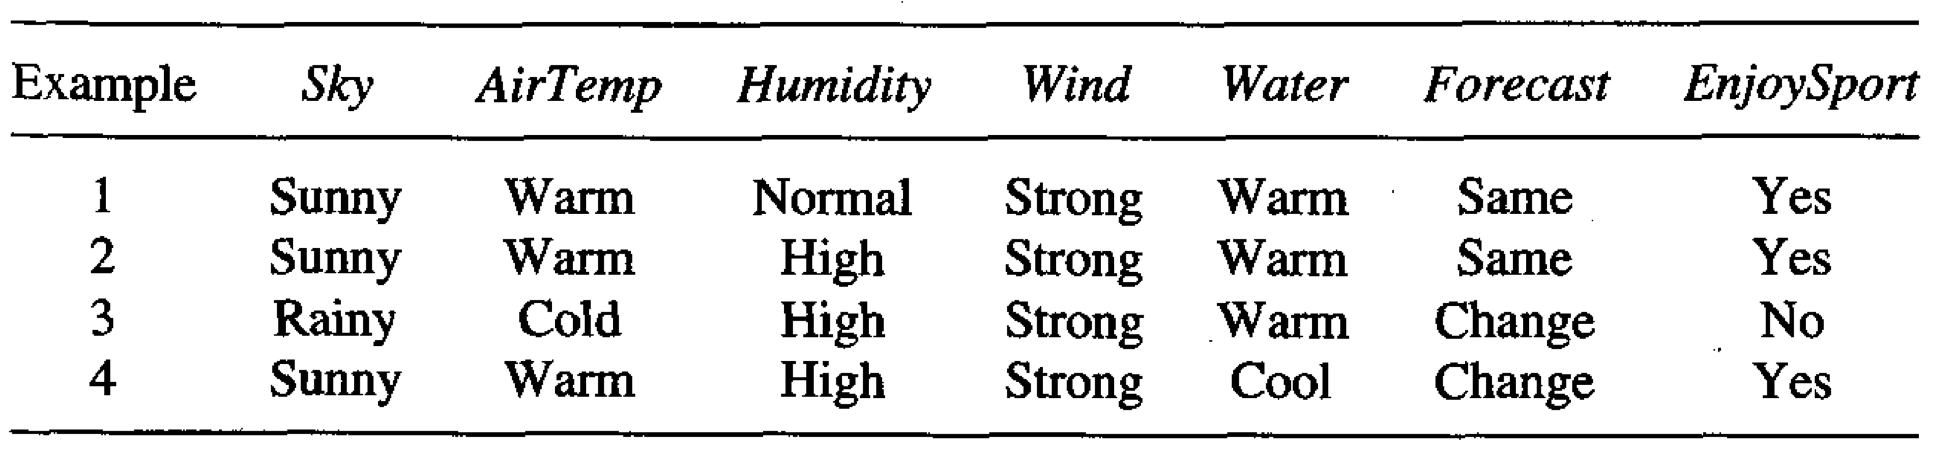
\includegraphics[width=0.9\textwidth]{enjoysport_examples}
\\from \cite{mitchell1997a}
\end{frame}

\begin{frame}{Hypothesis Space}
\begin{block}{How is the hypotheses space shaped?}
\begin{itemize}
\item the space of hypotheses is implicitly shaped by selecting the hypothesis representation
\item number of instances\footnote{distinct} in X: $3*2*2*2*2*2=96$ 
\item number of hypotheses\footnote{syntactically distinct} in H: $5*4*4*4*4*4=5120$
\end{itemize}
\end{block}
Many algorithms address learning by viewing it as \emph{searching the hypothesis space} in order to find hypotheses that best fit the data.
\end{frame}

\begin{frame}{General-to-specific ordering}
Example: 
\begin{itemize}
\item h1 = <Sunny, ?, ?, Strong, ?, ?>
\item h2 = <Sunny, ?, ?, ?, ?, ?>
\item h3 = <Sunny, ?, ?, ?, Cool, ?>
\end{itemize}

\begin{block}{More general than or equal to: ($\geq$)}
Let $h_j$ and $h_k$ be defined over X. Then $h_j \geq h_k$ iff: %i.e. <->
\centering $h_k(x) = 1 \Rightarrow h_j(x) = 1, \forall x \in X$
\end{block}

\begin{block}{More general to: ($>$)}
Let $h_j$ and $h_k$ be defined over X. Then $h_j > h_k$ iff:
\centering $h_j \geq h_k \land h_k \ngeq h_j$ %note: independent of x
\end{block}
\end{frame}

\begin{frame}{General-to-specific ordering}
\begin{itemize}
\item h1 = <Sunny, ?, ?, Strong, ?, ?>
\item h2 = <Sunny, ?, ?, ?, ?, ?>
\item h3 = <Sunny, ?, ?, ?, Cool, ?>
\end{itemize}

Verify the following expressions:
\begin{itemize}
\item $h2 > h1$? % true: h1 -> h2 AND it is not h2 -> h1 (for all x)
\item $h3 > h2$? % false: h3 NOT -> h2
\end{itemize}
\end{frame}

\begin{frame}{General-to-specific ordering}
\begin{itemize}
\item h1 = <Sunny, ?, ?, Strong, ?, ?>
\item h2 = <Sunny, ?, ?, ?, ?, ?>
\item h3 = <Sunny, ?, ?, ?, Cool, ?>
\end{itemize}

Verify the following expressions:
\begin{itemize}
\item $h2 > h1$? \textbf{true}, since h1 $\Rightarrow$ h2 AND it is NOT h2 $\Rightarrow$ h1 ($\forall $x)
\item $h3 > h2$? \textbf{false}, since h2 NOT $\Rightarrow$ h3 ($\exists$ x)
\end{itemize}
\end{frame}


\begin{frame}{General-to-specific ordering}
\begin{itemize}
\item h1 = <Sunny, ?, ?, Strong, ?, ?>
\item h2 = <Sunny, ?, ?, ?, ?, ?>
\item h3 = <Sunny, ?, ?, ?, Cool, ?>
\end{itemize}

Verify the following expressions:
\begin{itemize}
\item $h2 > h1$? \textbf{true}, since h1 $\Rightarrow$ h2 AND it is NOT h2 $\Rightarrow$ h1 ($\forall $x)
\item $h3 > h2$? \textbf{false}, since h2 NOT $\Rightarrow$ h3 ($\exists$ x)
\item $h3 \geq h1$? 
\end{itemize}
\end{frame}

\begin{frame}{General-to-specific ordering}
\begin{itemize}
\item h1 = <Sunny, ?, ?, Strong, ?, ?>
\item h2 = <Sunny, ?, ?, ?, ?, ?>
\item h3 = <Sunny, ?, ?, ?, Cool, ?>
\end{itemize}

Verify the following expressions:
\begin{itemize}
\item $h2 > h1$? \textbf{true}, since h1 $\Rightarrow$ h2 AND it is NOT h2 $\Rightarrow$ h1 ($\forall $x)
\item $h3 > h2$? \textbf{false}, since h2 NOT $\Rightarrow$ h3 ($\exists$ x)
\item $h3 \geq h1$? \textbf{false}, x=<Sunny, Warm, High, Strong, Warm, Same> $\Rightarrow h1(x)=1 \centernot \Rightarrow h3(x)=1$
\end{itemize}
\end{frame}

%% VISUALIZATION OF X AND H
\begin{frame}{Visualization of X and H}
\centering
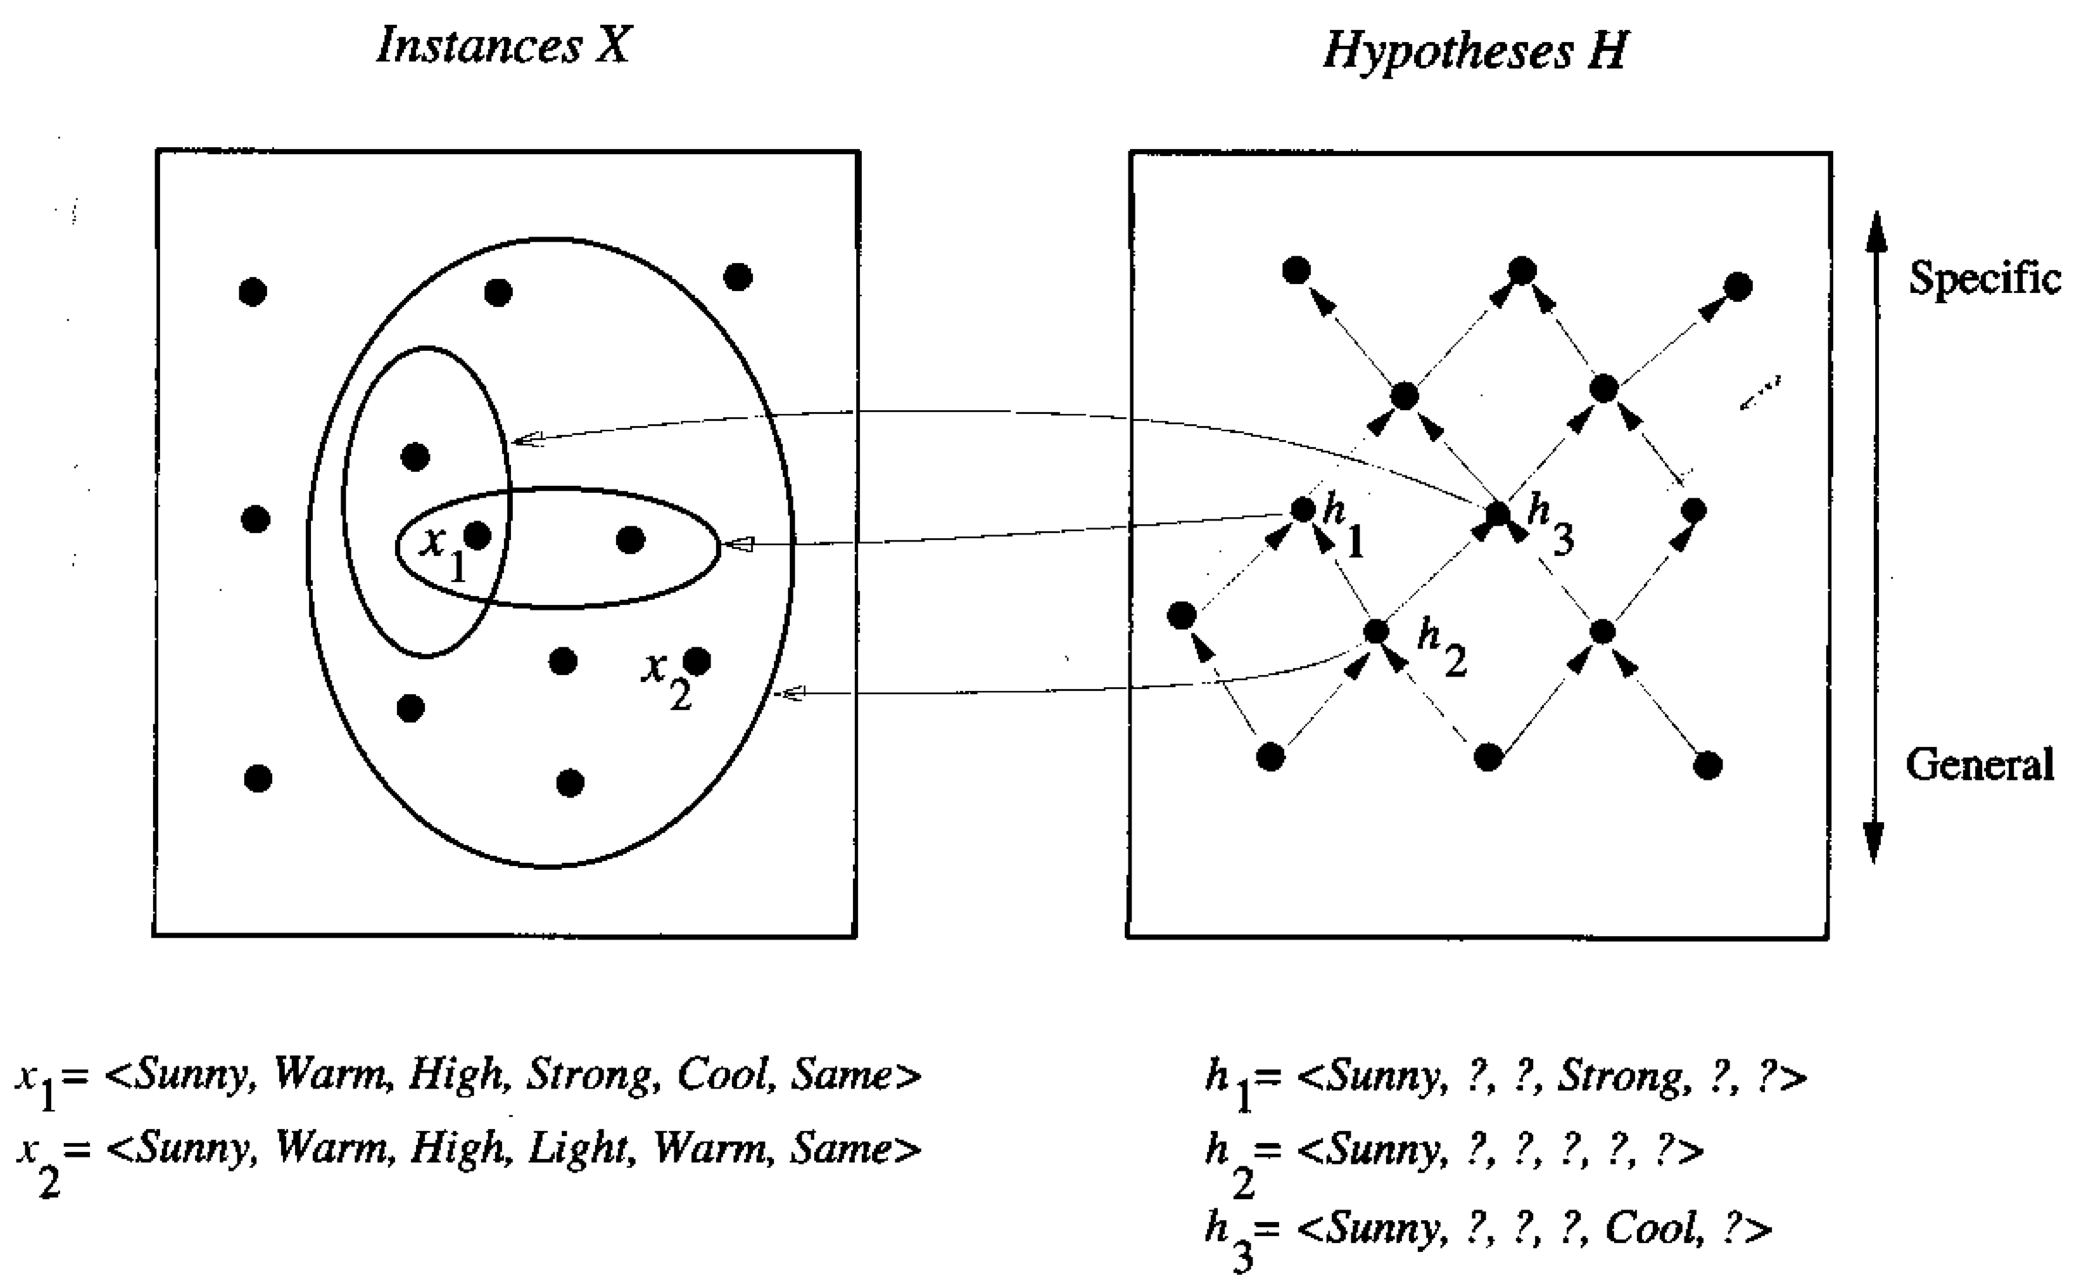
\includegraphics[width=0.9\textwidth]{X_and_H}
\\from \cite{mitchell1997a}
\end{frame}
\subsubsection{Algorithms}

\subsection{Learning as Search in the Hypothesis Space}
%% LEARNING AS SEARCH
\begin{frame}{Learning as Search in the Hypothesis Space}
\begin{enumerate}
\item Search from general to specific
	\begin{itemize}
	\item initial point is the most general hypothesis <?,...,?>
    \item positive samples are omitted
    \item negative samples are used for specialization
	\end{itemize}
\item Search from specific to general
	\begin{itemize}
	\item initial point is the most specific hypothesis <$\emptyset$,...,$\emptyset$>
    \item negative samples are omitted
    \item positive samples are used for generalization
	\end{itemize}
\item Combination of both: Candidate Elimination algorithm (later)
\end{enumerate}
\end{frame}


\begin{frame}{Learning as Search in the Hypothesis Space}
\begin{enumerate}
\item Search from general to specific
	\begin{itemize}
	\item initial point is the most general hypothesis <?,...,?>
    \item positive samples are omitted
    \item negative samples are used for specialization
	\end{itemize}
\item \textbf{Search from specific to general}
	\begin{itemize}
	\item initial point is the most specific hypothesis <$\emptyset$,...,$\emptyset$>
    \item negative samples are omitted
    \item positive samples are used for generalization
	\end{itemize}
\item Combination of both: Candidate Elimination algorithm (later)
\end{enumerate}
\end{frame}

\begin{frame}{Specific-to-General Algorithm}
\begin{enumerate}
\item initialize h as most specific hypothesis in H
\item for each positive training sample 
	\begin{itemize}
	\item for each attribute constraint $a_i$ in h <$a_0$,...,$a_n$>
    	\begin{itemize}
    	\item if $a_i$ is satisfied by x: do nothing
        \item else replace $a_i$ in h by the next more general constraint that is satisfied by x
    	\end{itemize}
	\end{itemize}
\item return hypothesis h
\end{enumerate}
\end{frame}

\begin{frame}{Specific-to-General Algorithm (2)}
\centering
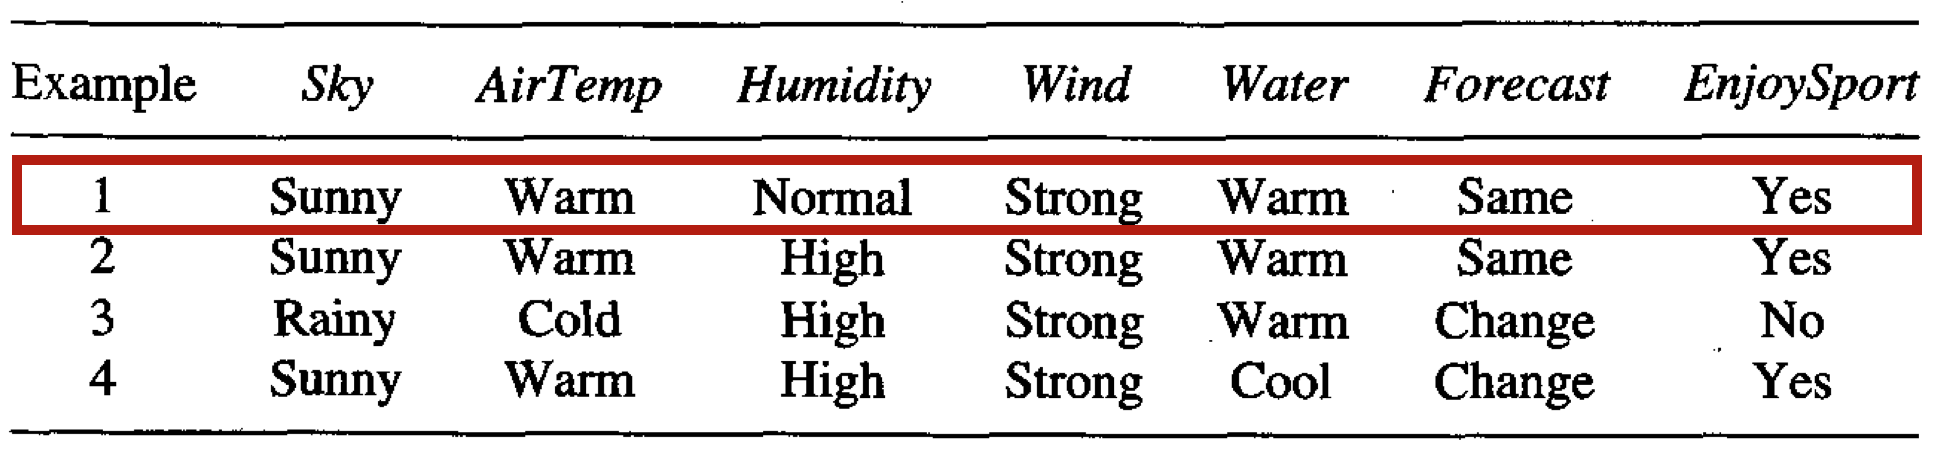
\includegraphics[width=0.9\textwidth]{enjoysport_examples_1}
\begin{itemize}
\item initialization: h=$<\emptyset,\emptyset,\emptyset,\emptyset,\emptyset,\emptyset>$
\item first sample is positive (EnjoySport($x_1$) = true)
\item However, h($x_1$)=false $\rightarrow$ generalize
\item h=<Sunny, Warm, Normal, Strong, Warm, Same> %next general constraint that is satisfied with x1
\end{itemize}
\end{frame}

\begin{frame}{Specific-to-General Algorithm (3)}
\centering
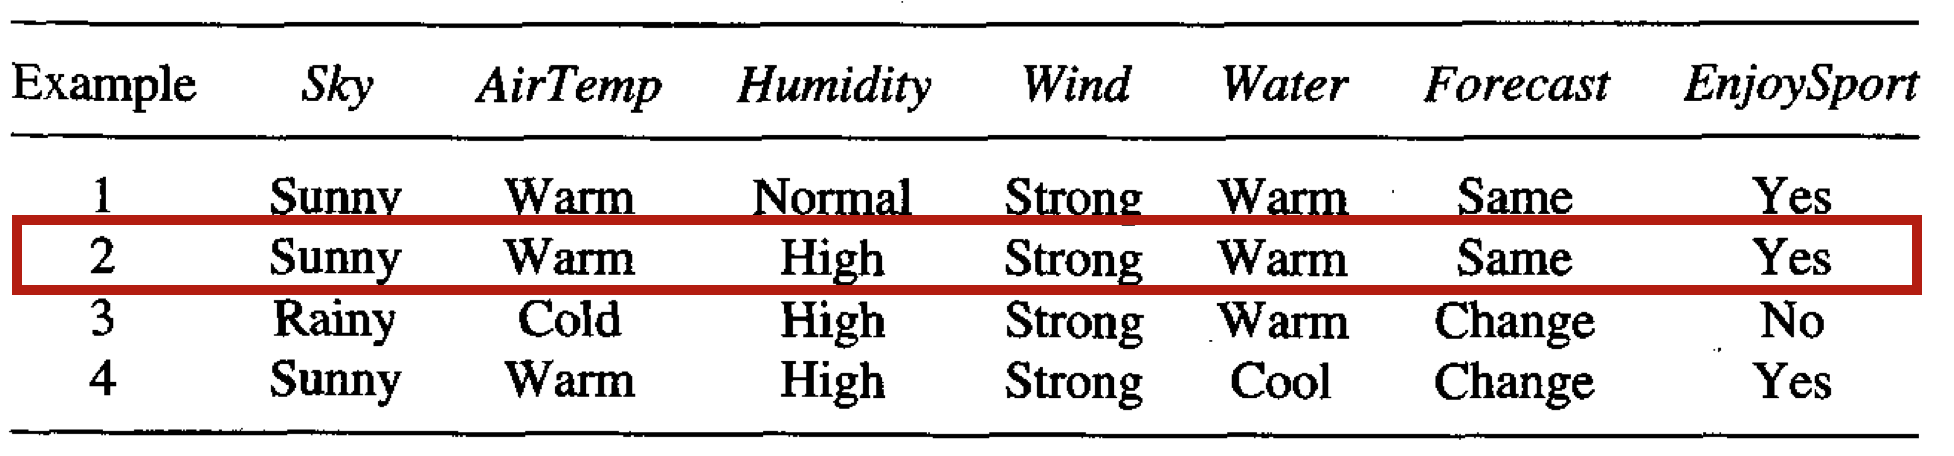
\includegraphics[width=0.9\textwidth]{enjoysport_examples_2}
\begin{itemize}
\item h=<Sunny, Warm, Normal, Strong, Warm, Same>
\item second sample is positive
\item However, h($x_2$)=false $\rightarrow$ generalize (minimally)
\item h=<Sunny, Warm, ?, Strong, Warm, Same> %next general constraint that is satisfied with x2
\end{itemize}
\end{frame}

\begin{frame}{Specific-to-General Algorithm (4)}
\centering
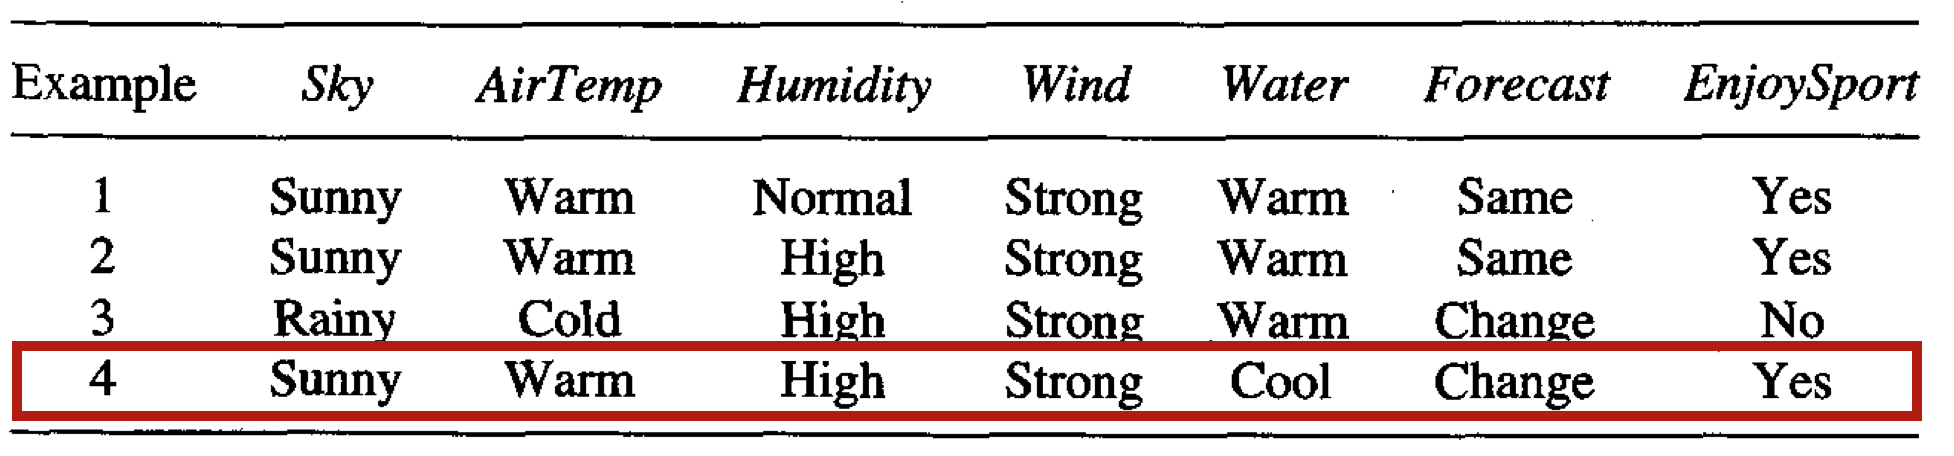
\includegraphics[width=0.9\textwidth]{enjoysport_examples_3}
\begin{itemize}
\item h=<Sunny, Warm, ?, Strong, Warm, Same>
\item third sample is negative (EnjoySport($x_3$) = false) $\rightarrow$ \textbf{ignored}
\end{itemize}

\begin{itemize}
\item forth sample is positive
\item However, h($x_2$)=false $\rightarrow$ generalize (minimally)
\item \textbf{h=<Sunny, Warm, ?, Strong, ?, ?>} %next general constraint that is satisfied with x2
\item termination, return h
\end{itemize}
\end{frame}

\begin{frame}{Specific-to-General Algorithm (5)}
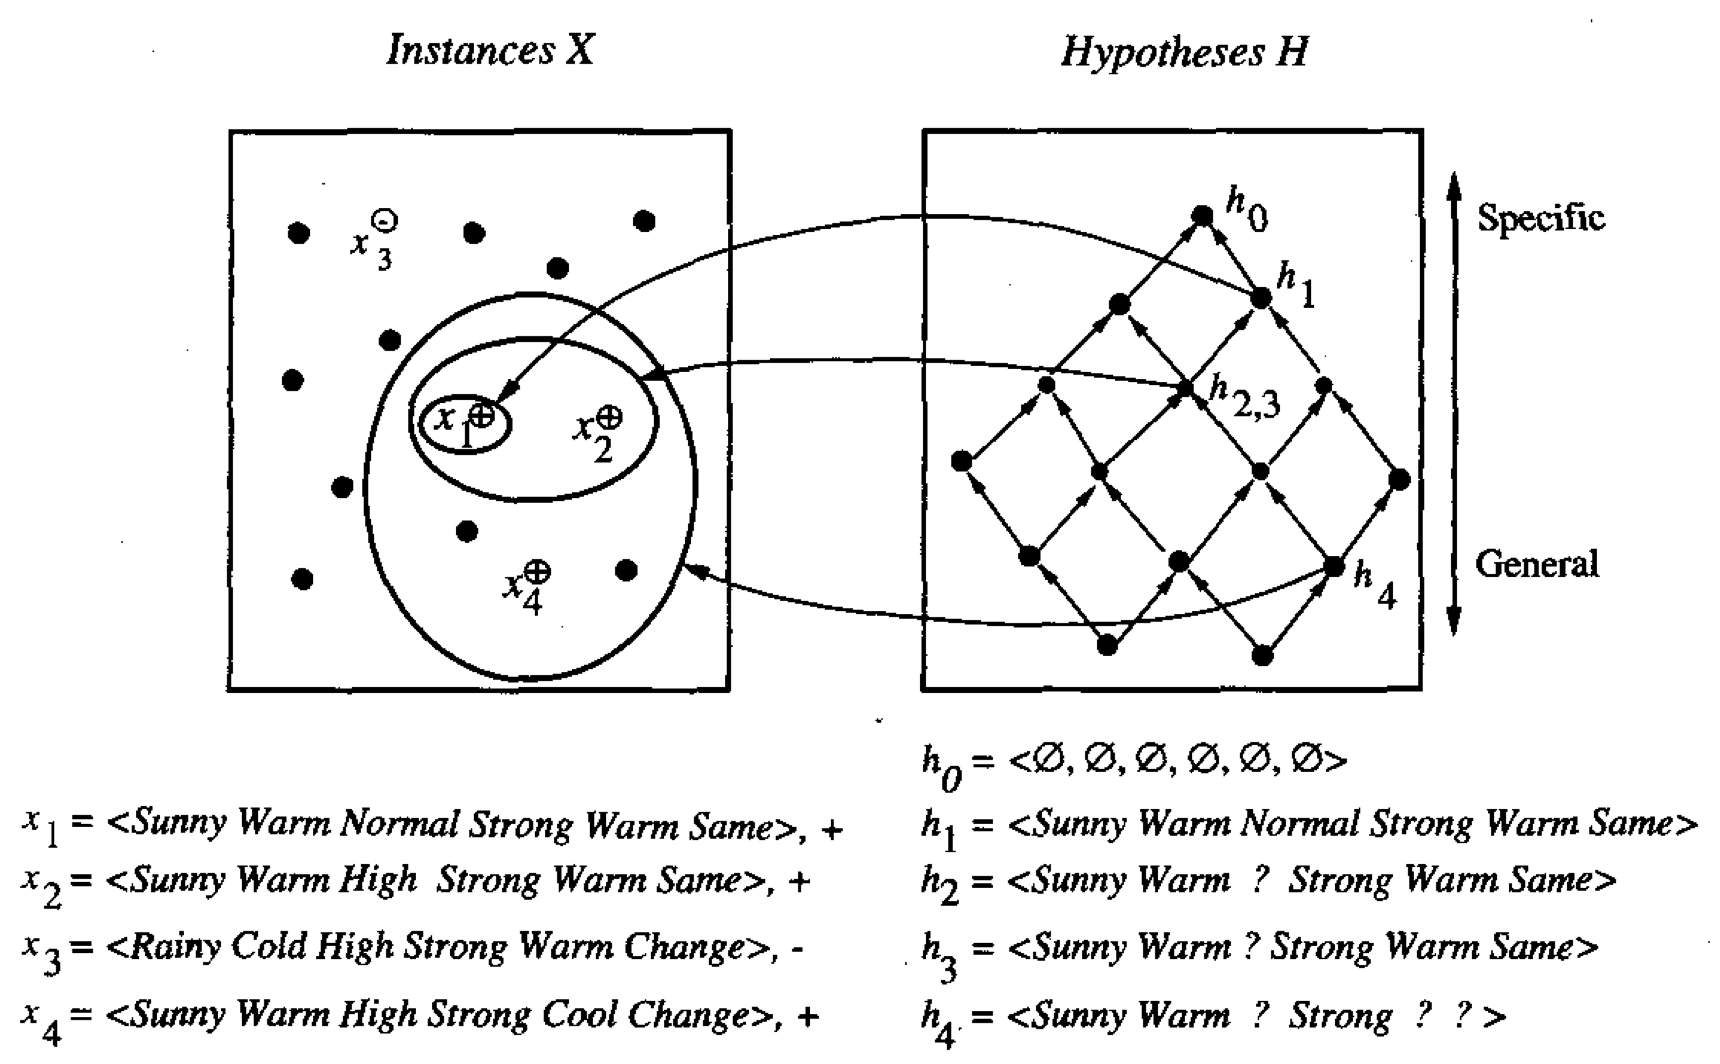
\includegraphics[width=0.9\textwidth]{X_and_H_1}
\end{frame}

\begin{frame}{Specific-to-general Algorithm (5)}
\begin{block}{Properties of the Specific-to-General Algorithm}
\begin{itemize}
\item algorithm is \textbf{guaranteed to output the most specific hypothesis} within H that is consistent with the positive training samples
% definition consistency: no negative samples are classified positive, all positive samples are classified positive
\item final hypothesis is also \textbf{consistent with negative samples} provided
\begin{itemize}
\item the correct target concept is in H
\item the examples are correct
\end{itemize}
\end{itemize}
\end{block}
\end{frame}



\begin{frame}{Specific-to-general Algorithm (5)}
\begin{block}{Properties of the Specific-to-General Algorithm}
\begin{itemize}
\item algorithm is \textbf{guaranteed to output the most specific hypothesis} within H that is consistent with the positive training samples
% definition consistency: no negative samples are classified positive, all positive samples are classified positive
\item final hypothesis is also \textbf{consistent with negative samples} provided
\begin{itemize}
\item the correct target concept is in H
\item the examples are correct
\end{itemize}
\end{itemize}
\end{block}
\textbf{BUT:}
\begin{itemize}
\item is the found \emph{h} the only one consistent with the data?
\item why prefer the most specific \emph{$h_{specific}$}? Unclear whether we should prefer it over the most general \emph{$h_{general}$}.
\item data-inefficient (negative samples ignored) ... and more
\end{itemize}
\end{frame}



\begin{frame}{Version Space and Candidate Elimination Algorithm}
\begin{block}{Candidate Elimination algorithm}
The Candidate Elimination algorithm finds all describable hypotheses that are consistent with the observed training examples.
\end{block}
$\rightarrow$ represents the set of \emph{all} hypotheses consistent with the observed data. This set is called \emph{Version Space}

\begin{block}{Version Space?}
The version space, denoted $VS_{H,D}$, with respect to hypothesis space H and training examples D, is the subset of hypotheses from H \emph{consistent} with the training examples in D.
\end{block}
\cite{russel2003,mitchell1997a}
\end{frame}



\begin{frame}{Example of the Version Space (2)}
\centering
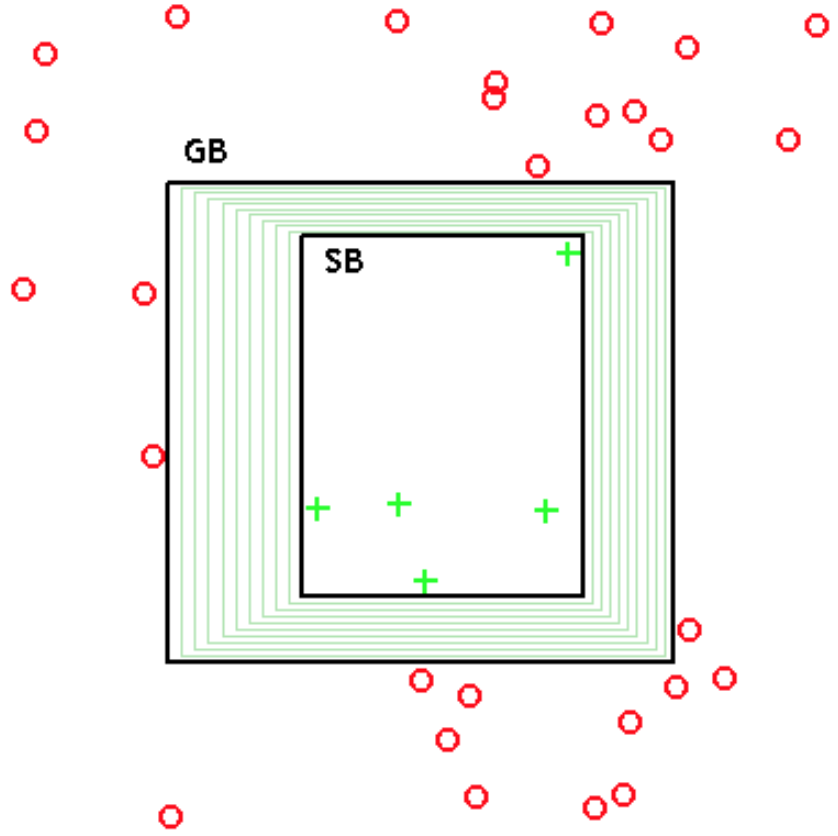
\includegraphics[width=0.5\textwidth]{version_space}
\\GB = maximally \textbf{general} positive boundary, SB = maximally \textbf{specific} positive boundary %hypotheses are intermediate thin rectangles
\cite{Dfass2006}
\end{frame}


\begin{frame}{Example of the Version Space (2)}
\centering
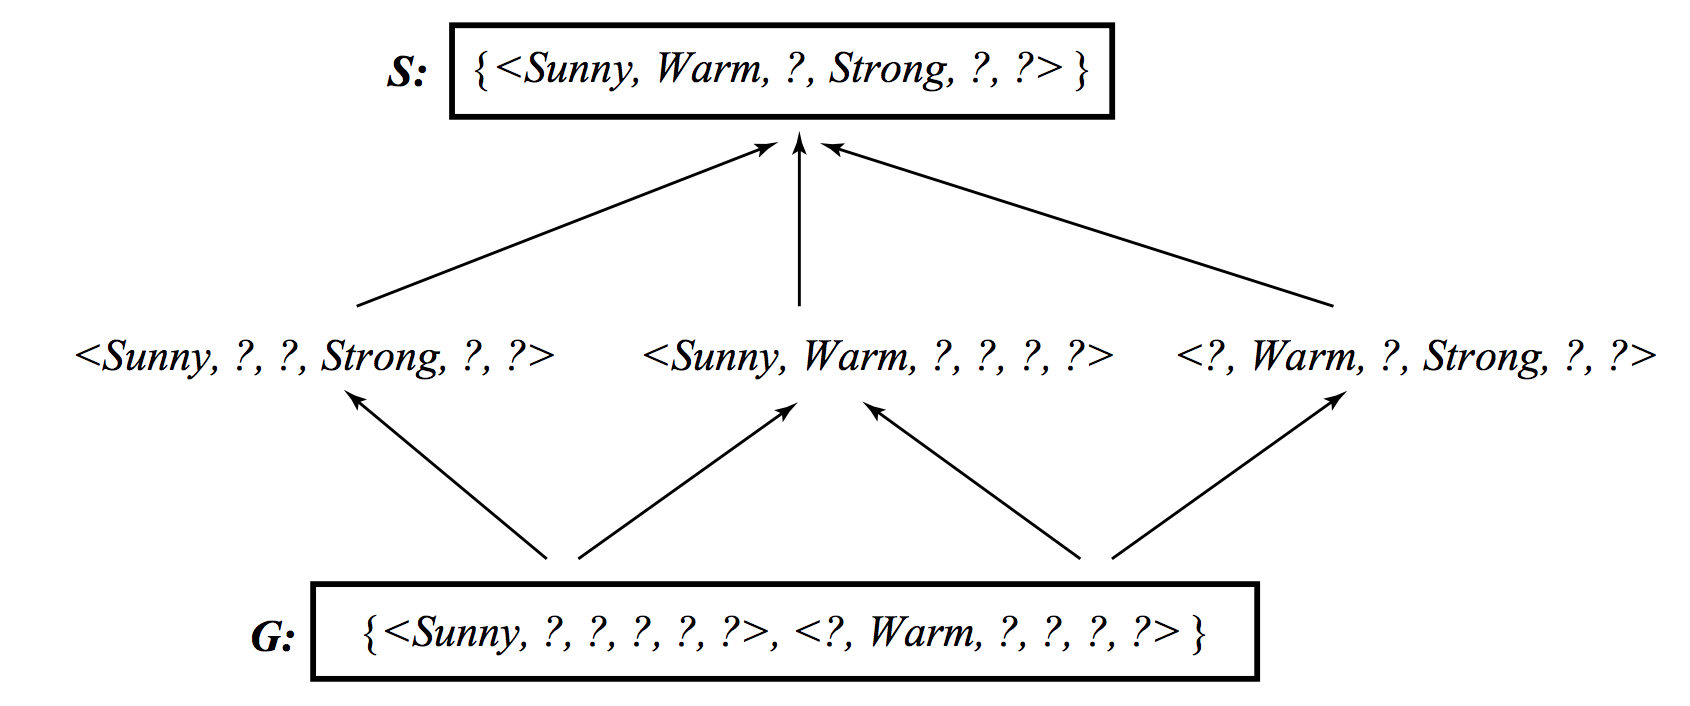
\includegraphics[width=0.9\textwidth]{version_space_1}
\\The version space for the \emph{EnjoySports} concept learning task with the previously shown samples. The VS includes all six hypotheses. However, it can simply represented by G and S.
\end{frame}


\begin{frame}{Candidate Elimination Algorithm}
Preliminary:
\begin{itemize}
\item S = $\{$\emph{s} | \emph{s} being a hypothesis consistent with the observed samples $\land$ there exists no hypothesis which is more \textbf{specific} than \emph{s} that is also consistent with all samples$\}$
\item initialize S with $<\emptyset>$ 
\item G = $\{$\emph{g} | \emph{g} being a hypothesis consistent with the observed samples $\land$ there exists no hypothesis which is more \textbf{general} than \emph{g} that is also consistent with all samples$\}$
\item initialize G with $<?>$
\end{itemize}
\end{frame}


\begin{frame}{Candidate Elimination Algorithm (2)}

\begin{columns}
\begin{column}{0.5\textwidth}
\textbf{\color{brown}x is a negative sample:}
\begin{itemize}
\item remove from \emph{S} any hypothesis inconsistent with x
\item for each hypothesis \emph{g} in \emph{G} inconsistent with x: 
  \begin{itemize}
  \item remove \emph{g} from \emph{G} 
  \item add to \emph{G} all minimal specializations \emph{h} s.t. \emph{h} is consistent with x, and some member of \emph{S} is more specific than \emph{h}
  \end{itemize}
\item remove from \emph{G} any hypothesis less general than another hypothesis in \emph{G}
\end{itemize}	
\end{column}
\begin{column}{0.5\textwidth}
\end{column}
\end{columns}

\end{frame}



\begin{frame}{Candidate Elimination Algorithm (2)}

\begin{columns}
\begin{column}{0.55\textwidth}
\textbf{\color{brown}x is a negative sample:}
\begin{itemize}
\item \textbf{remove from \emph{S}} any hypothesis inconsistent with x
\item for each hypothesis \emph{g} in \emph{G} inconsistent with x: 
  \begin{itemize}
  \item \textbf{remove \emph{g} from \emph{G}}
  \item \textbf{add to \emph{G}} all minimal \textbf{specializations} \emph{h} of \emph{S} s.t. \emph{h} is consistent with x, and some member of \emph{S} is more \textbf{specific} than \emph{h}
  \end{itemize}
\item \textbf{remove from \emph{G}} any hypothesis less general than another hypothesis in \emph{G}
\end{itemize}	
\end{column}
\begin{column}{0.55\textwidth}
\textbf{\color{blue}x is a positive sample:}
\begin{itemize}
\item \textbf{remove from \emph{G}} any hypothesis inconsistent with x
\item for each hypothesis \emph{s} in \emph{S} inconsistent with x:
	\begin{itemize}
	\item \textbf{remove \emph{s} from \emph{S}}
    \item \textbf{add to \emph{S}} all minimal \textbf{generalizations} \emph{h} of \emph{S} s.t. \emph{h} is consistent with x, and some member of G is more \textbf{general} than \emph{h}
	\end{itemize}
\item \textbf{remove from \emph{S}} any hypothesis less general than other hypothesis in \emph{S}
\end{itemize}
\end{column}
\end{columns}
\end{frame}

\begin{frame}{Candidate Elimination Algorithm Example}
\centering
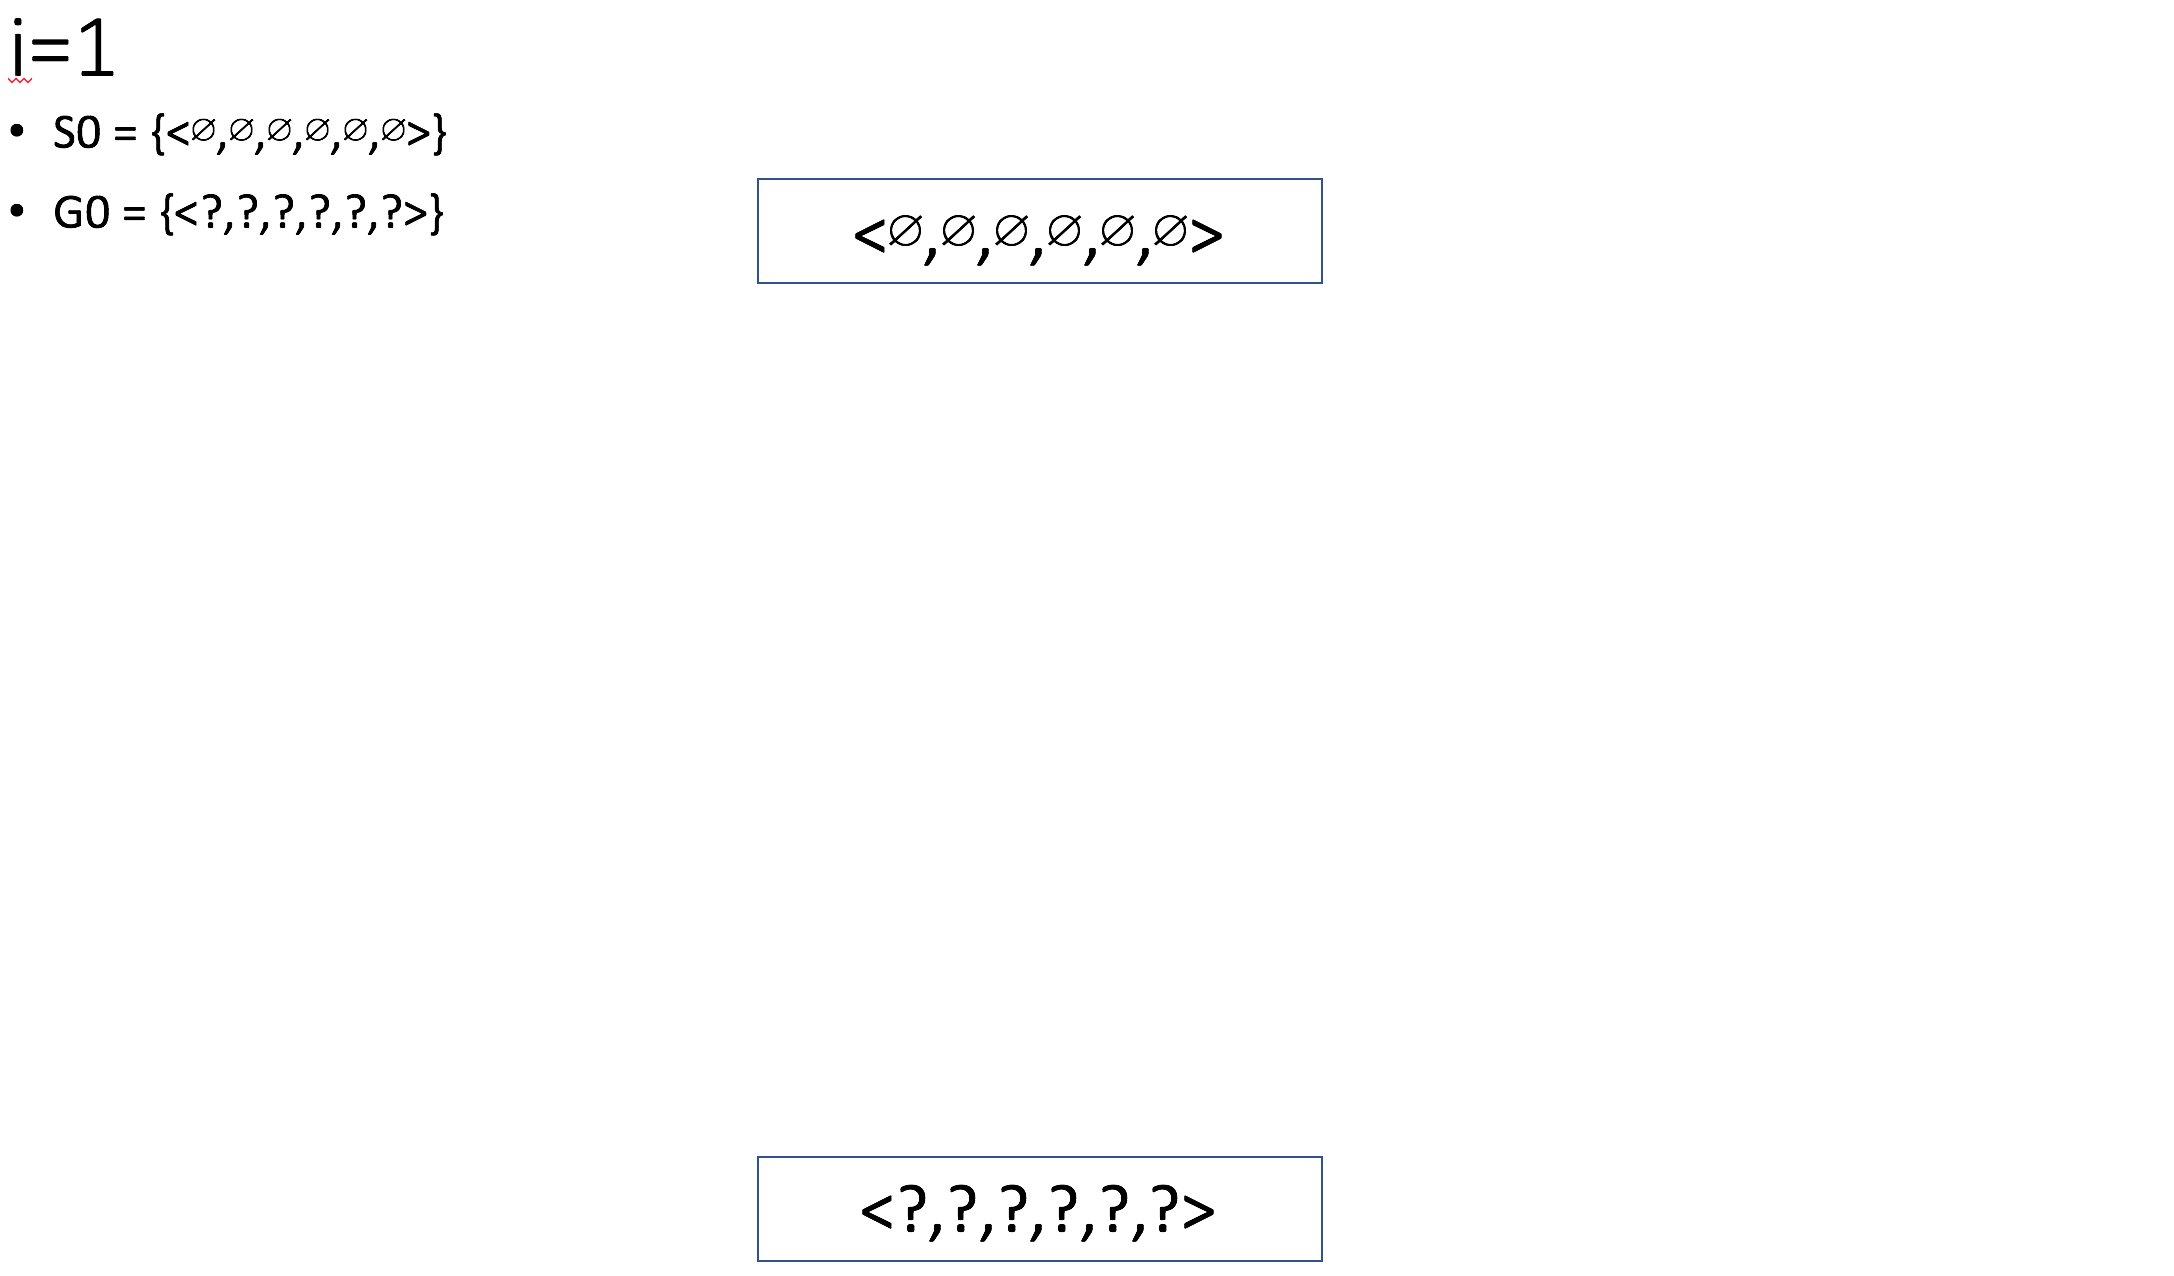
\includegraphics[width=1.1\textwidth]{cea_1}
\end{frame}

\begin{frame}{Candidate Elimination Algorithm Example}
\centering
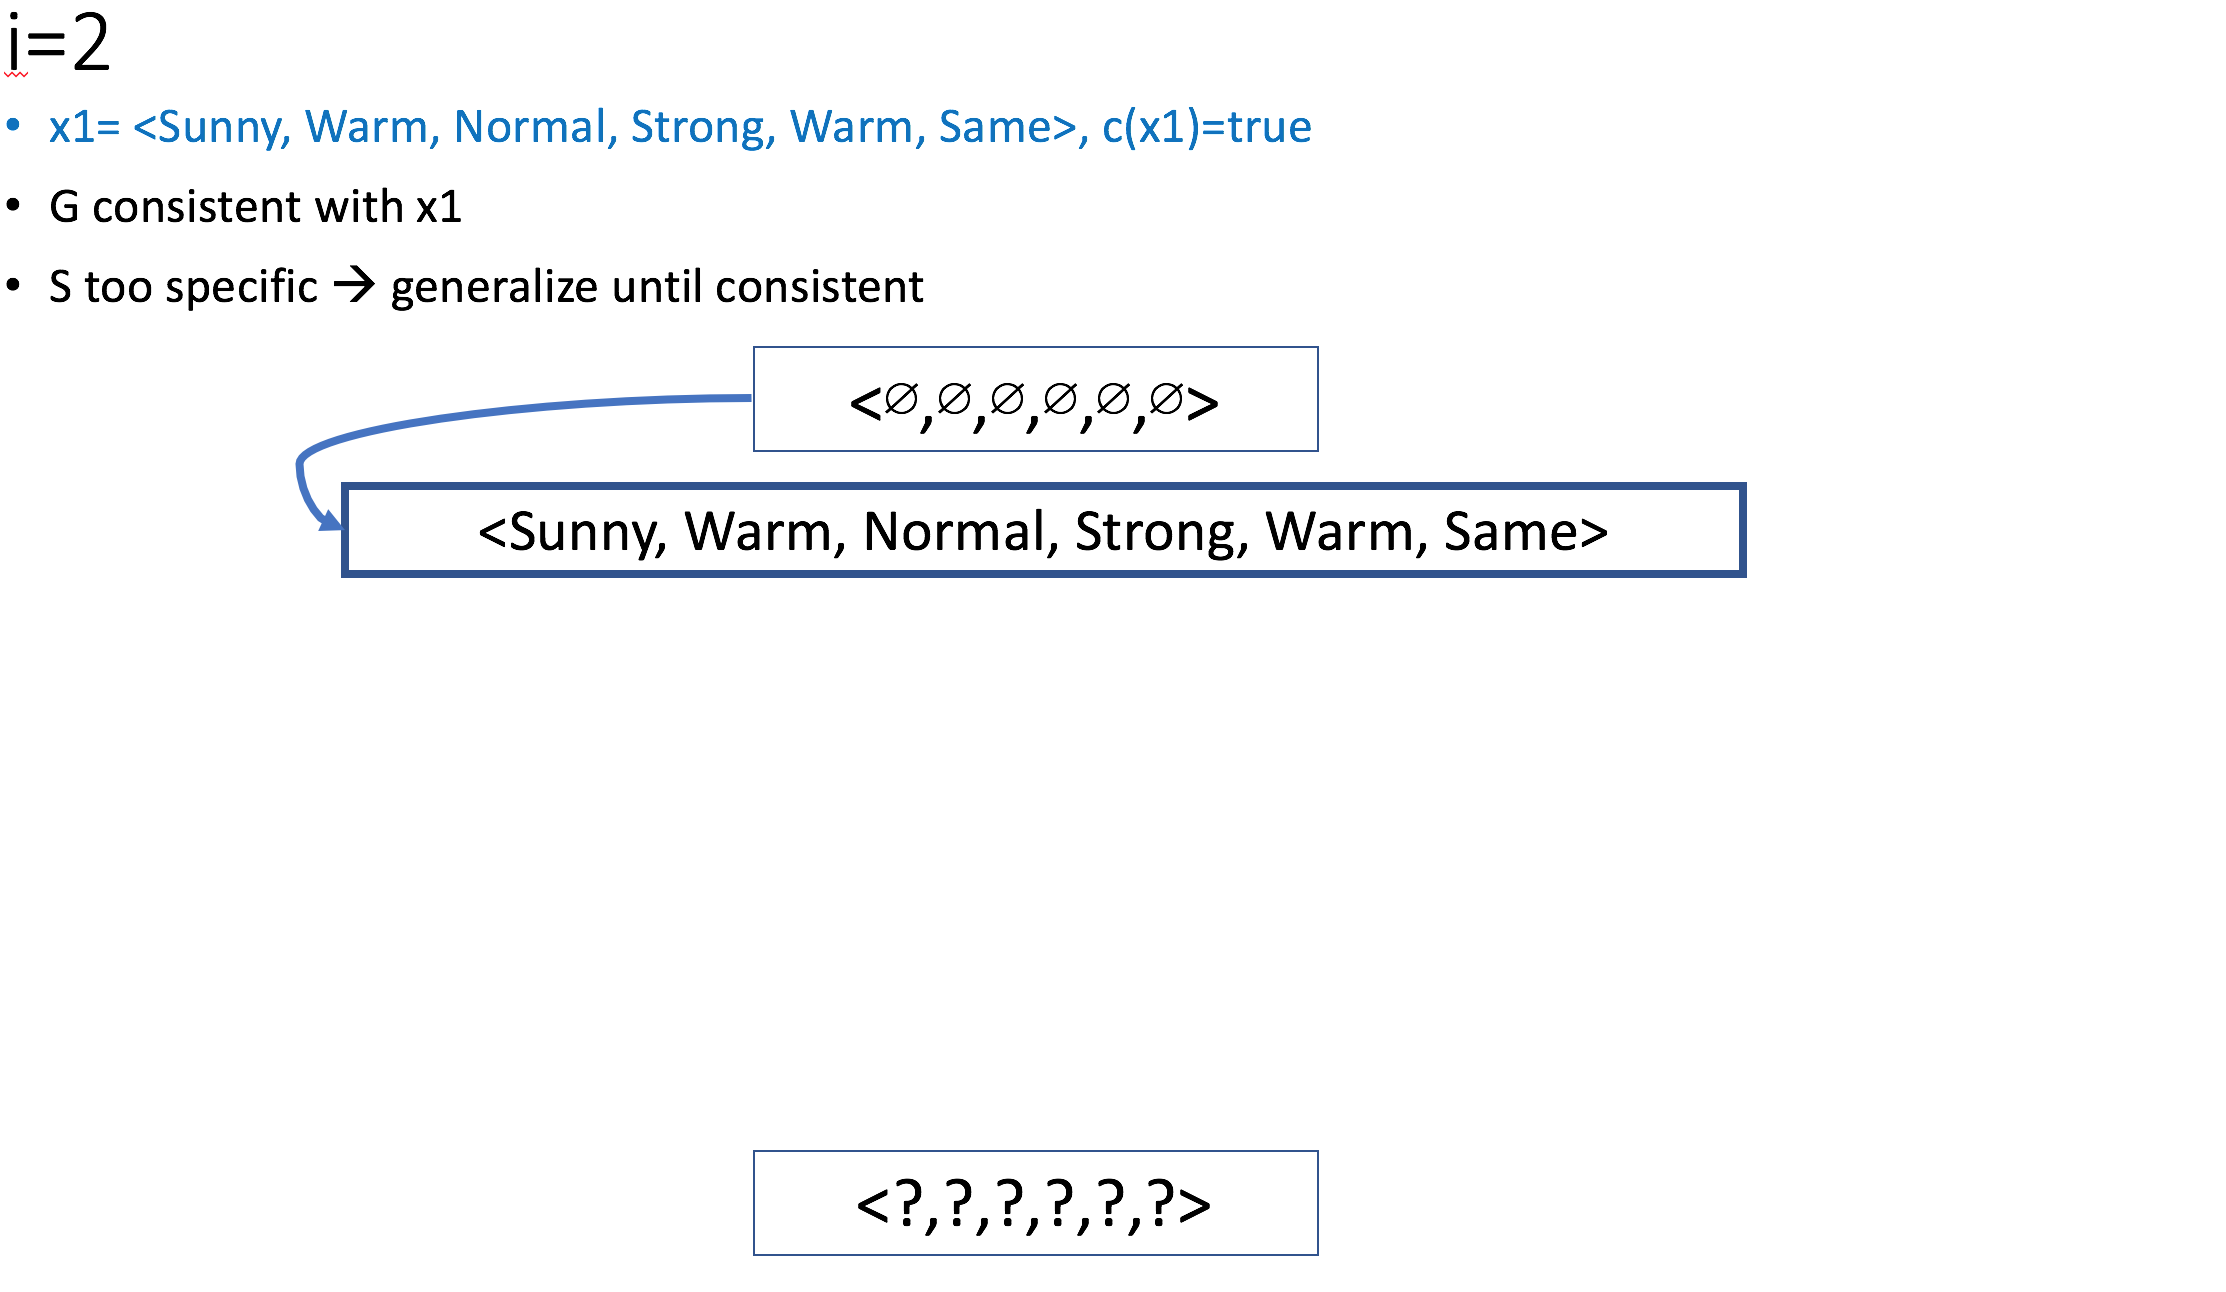
\includegraphics[width=1.1\textwidth]{cea_2}
\end{frame}

\begin{frame}{Candidate Elimination Algorithm Example}
\centering
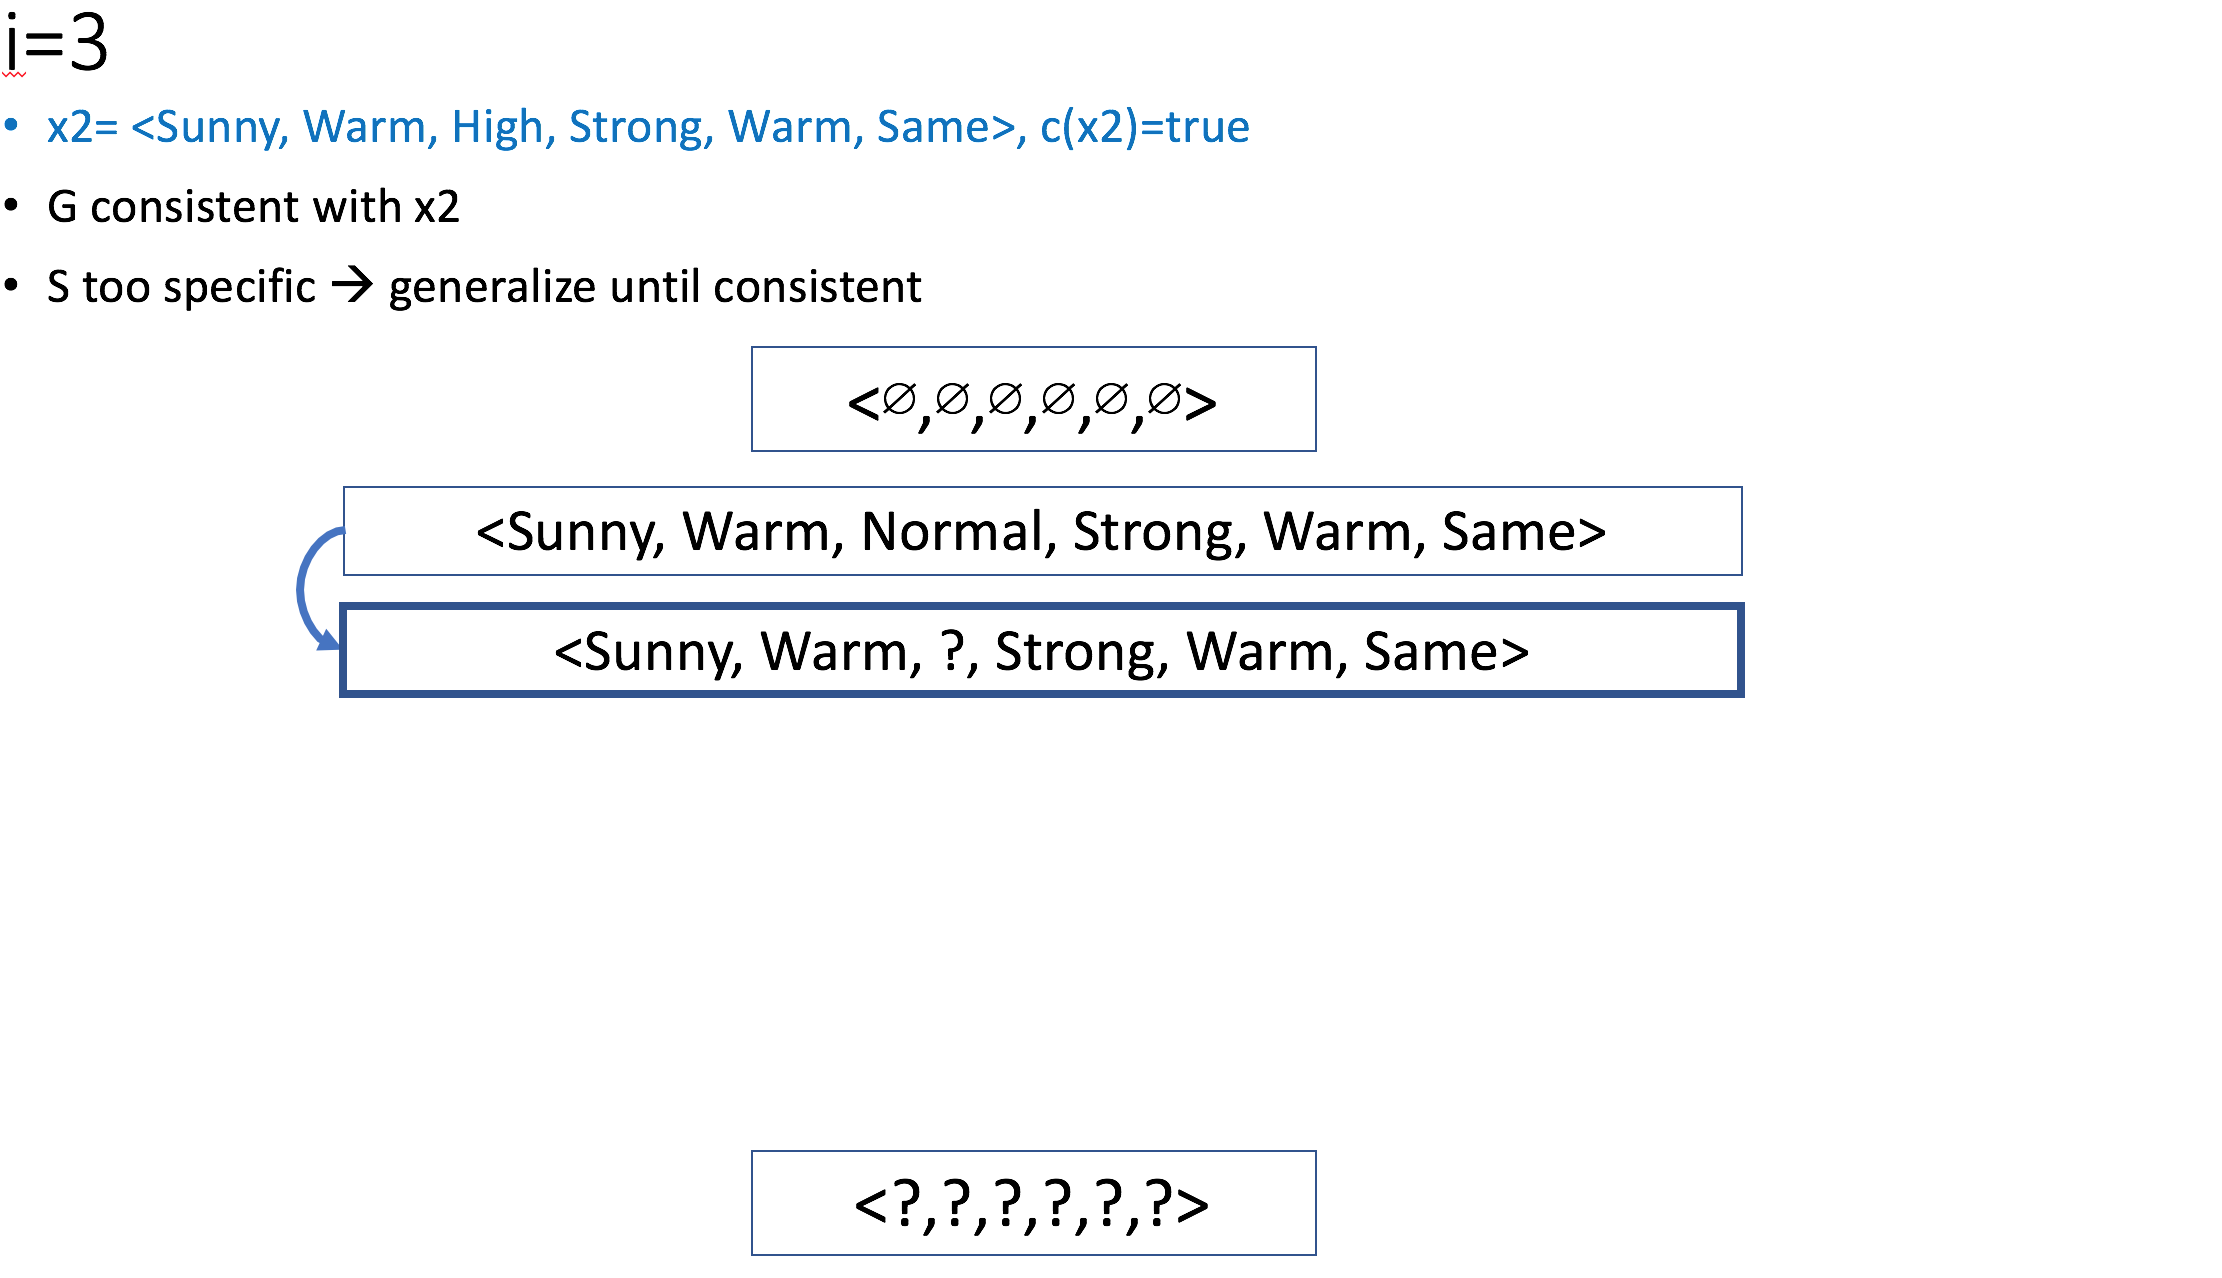
\includegraphics[width=1.1\textwidth]{cea_3}
\end{frame}

\begin{frame}{Candidate Elimination Algorithm Example}
\centering
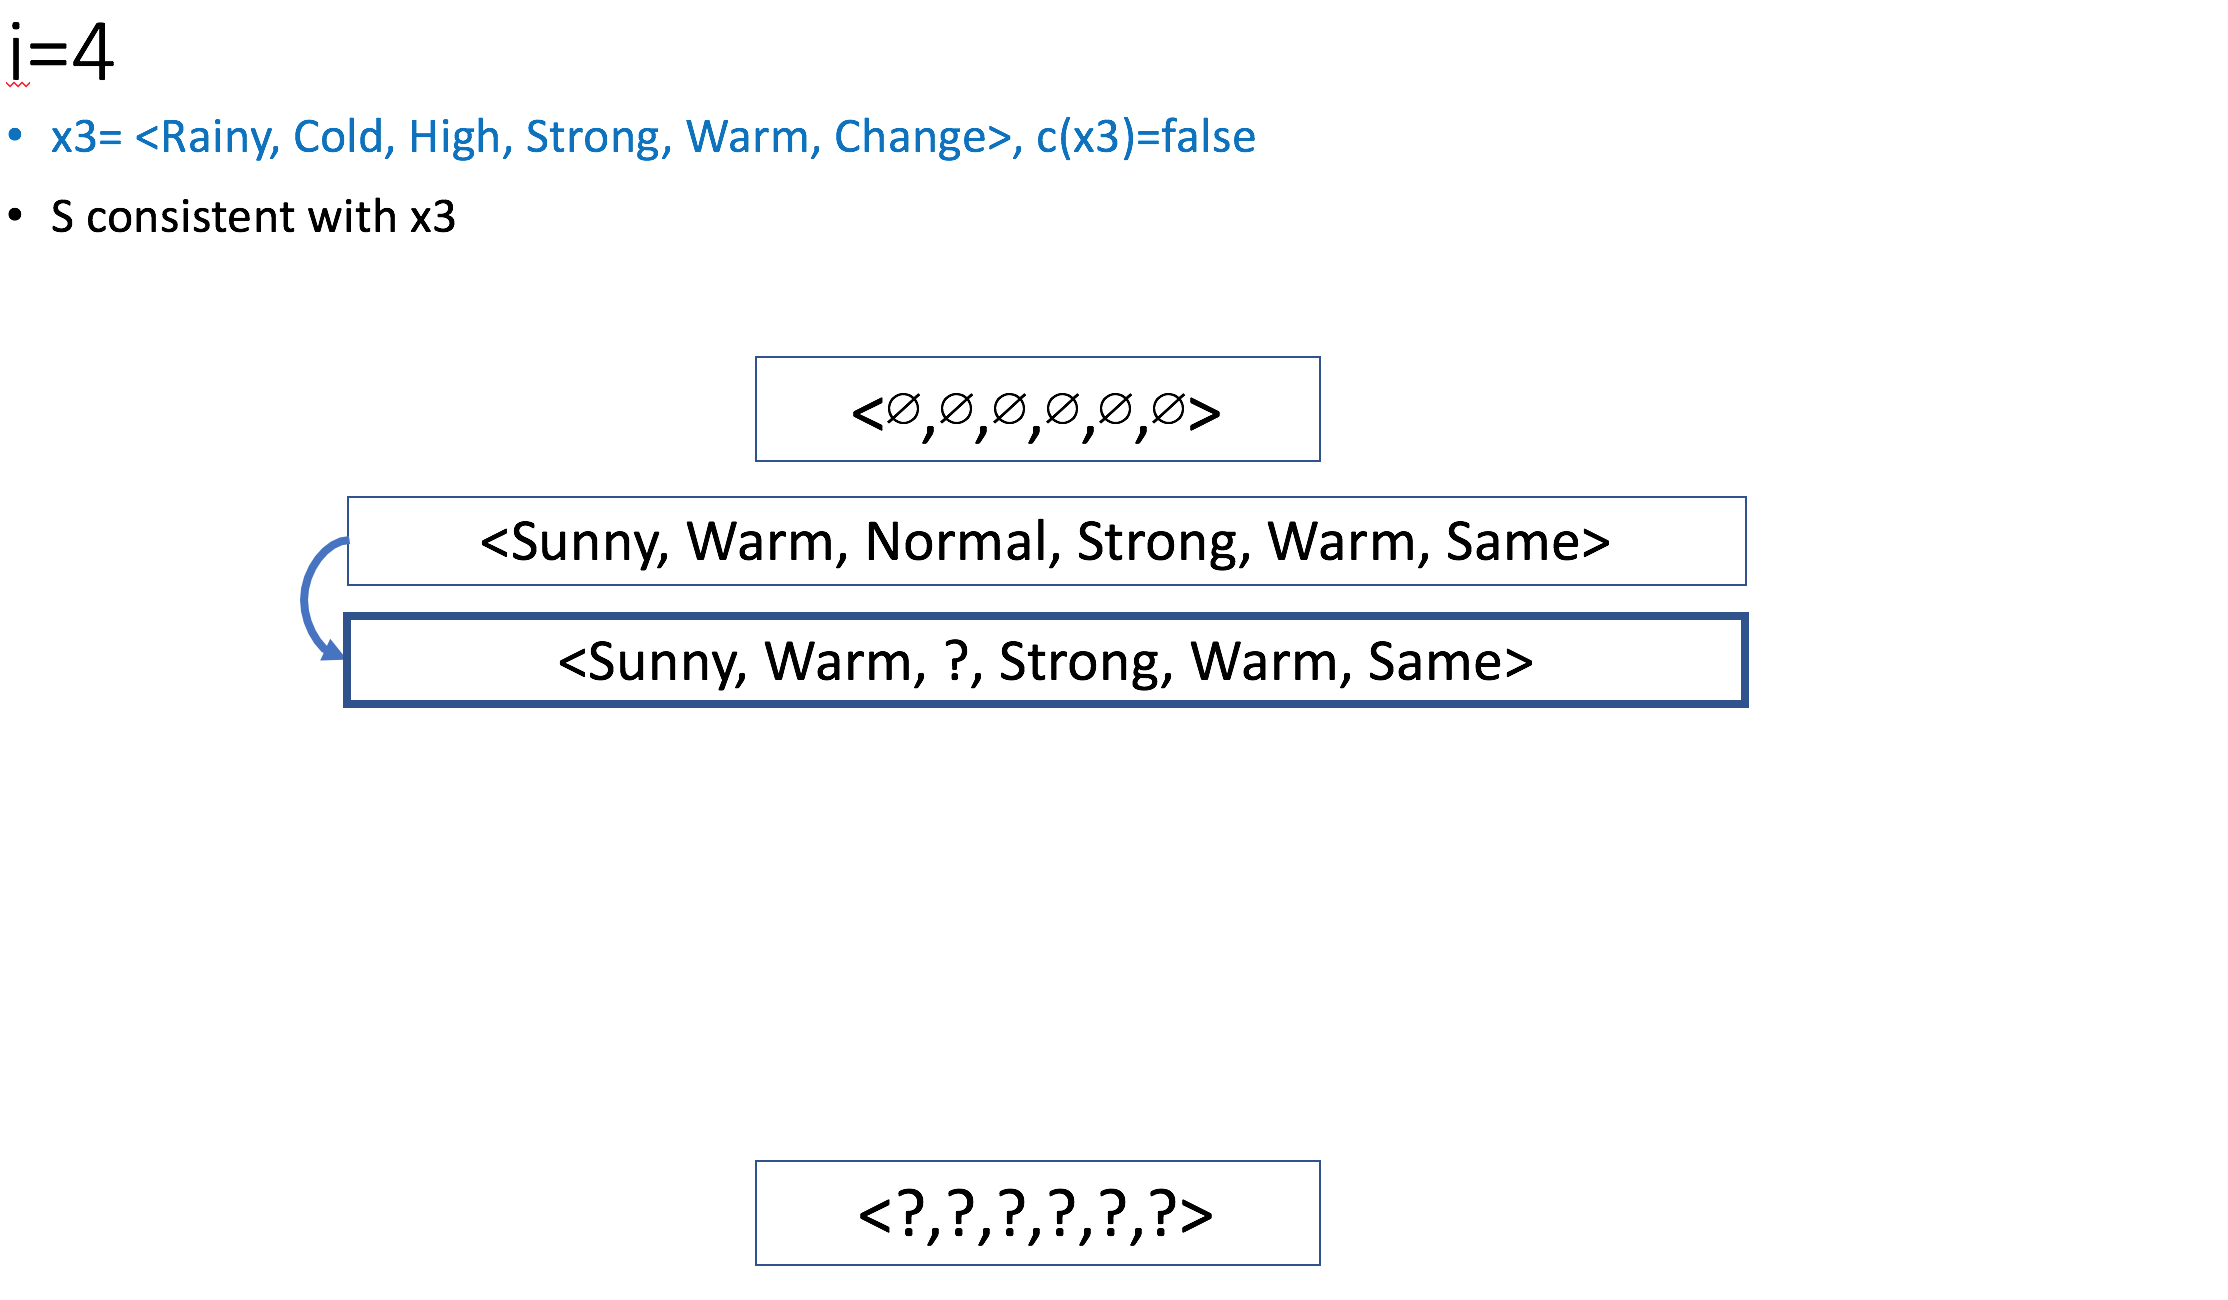
\includegraphics[width=1.1\textwidth]{cea_4}
\end{frame}

\begin{frame}{Candidate Elimination Algorithm Example}
\centering
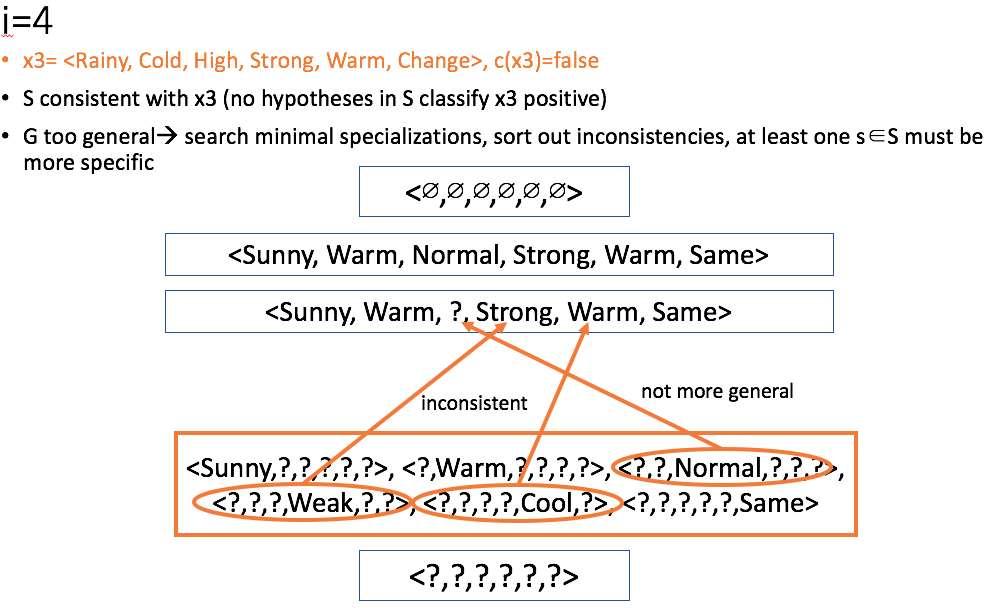
\includegraphics[width=1\textwidth]{cea_5}
\end{frame}

\begin{frame}{Candidate Elimination Algorithm Example}
\centering
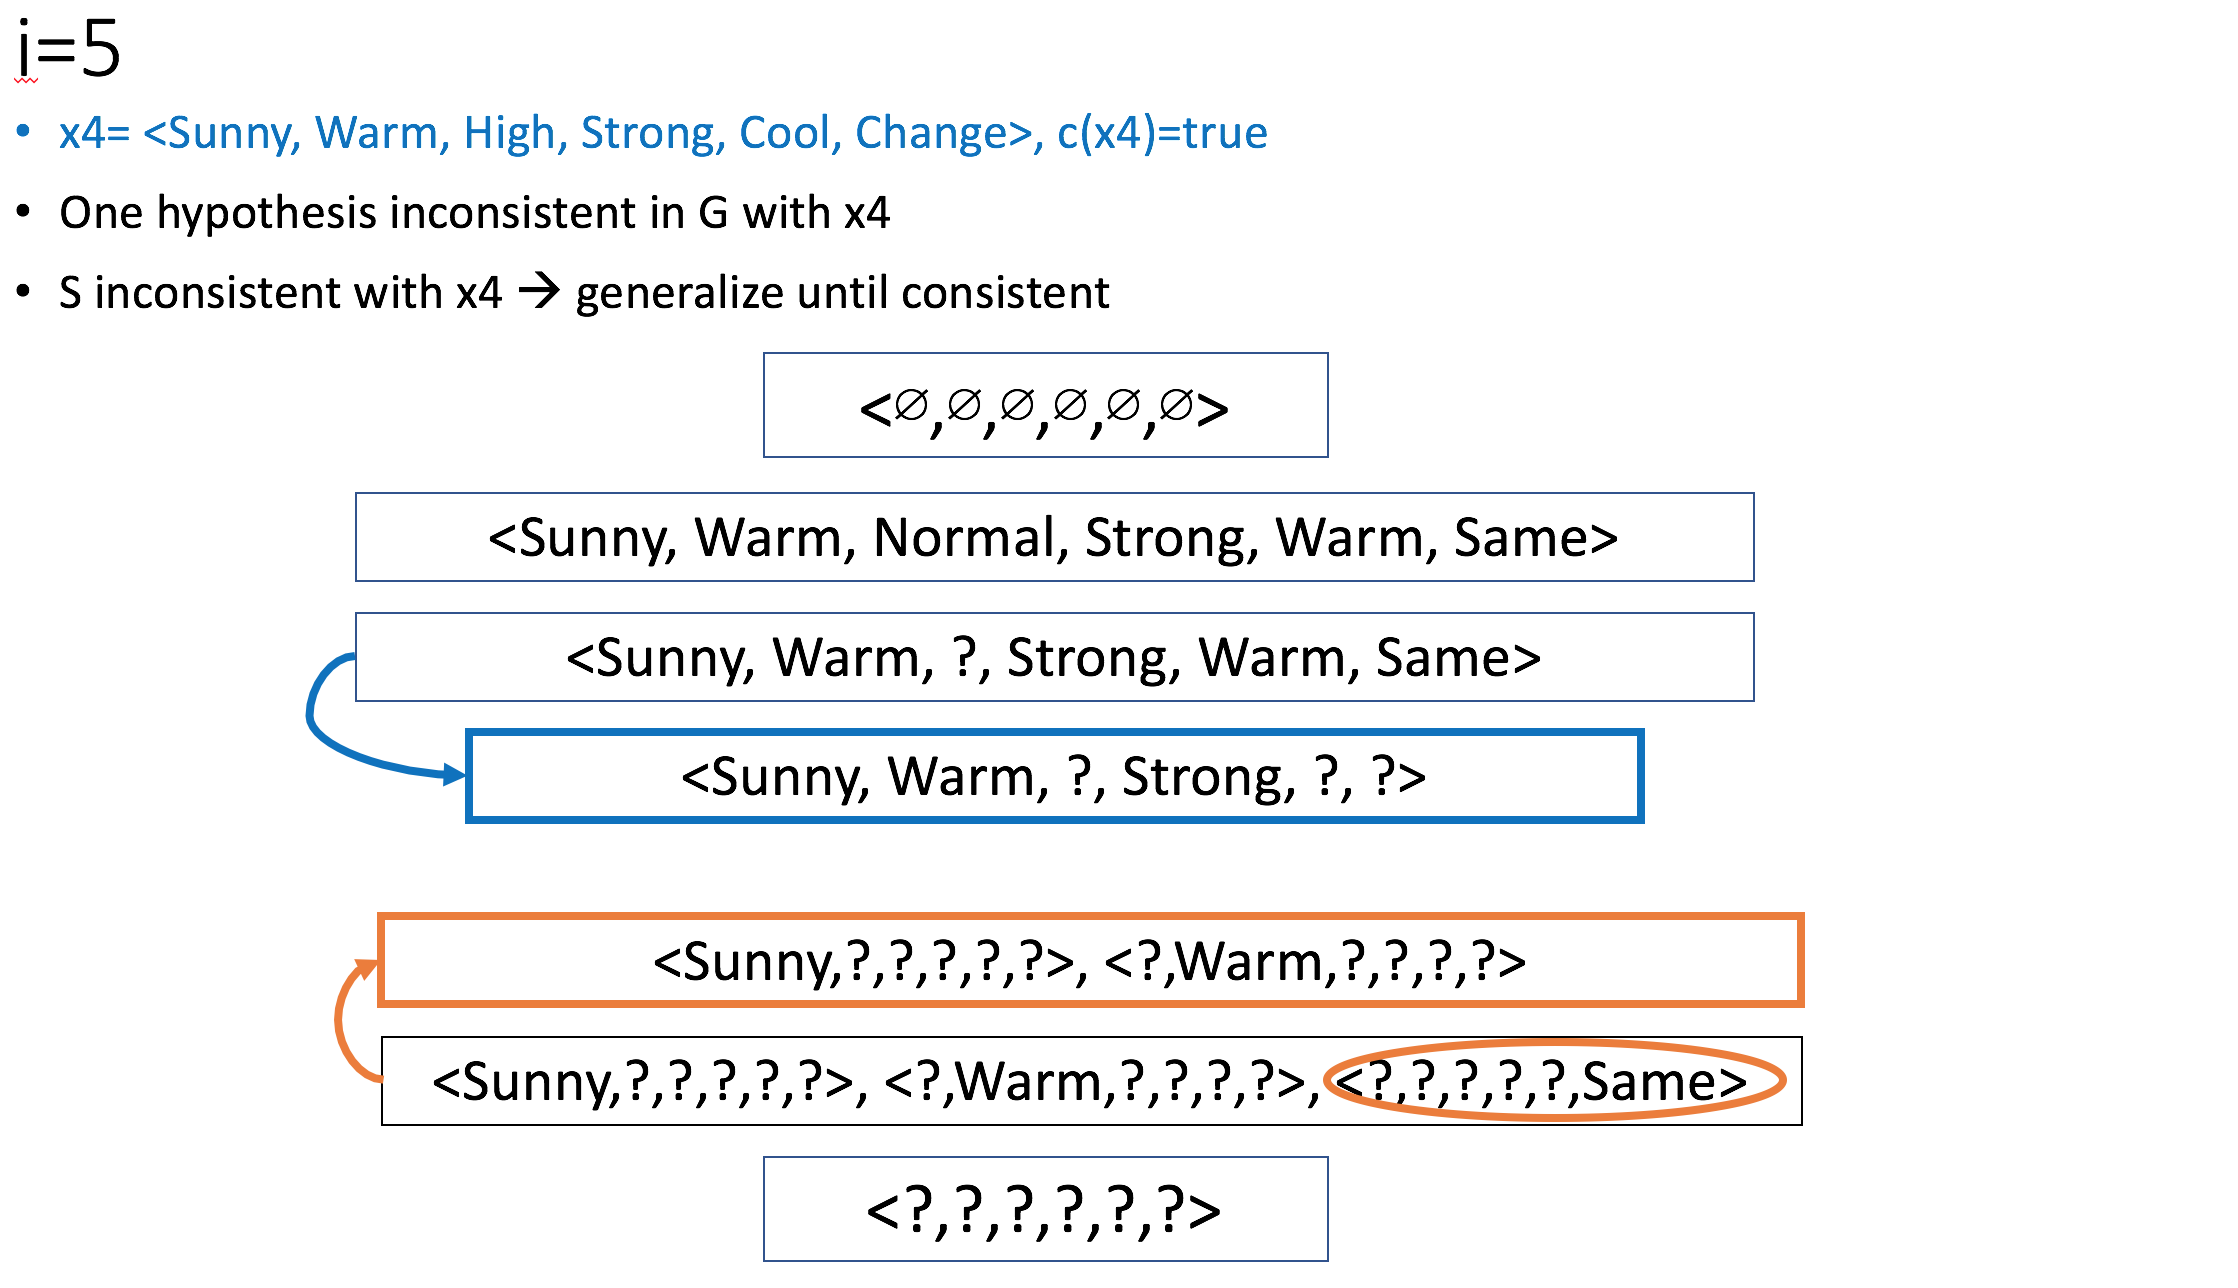
\includegraphics[width=1.1\textwidth]{cea_6}
\end{frame}

\begin{frame}{Candidate Elimination Algorithm Example}
\centering
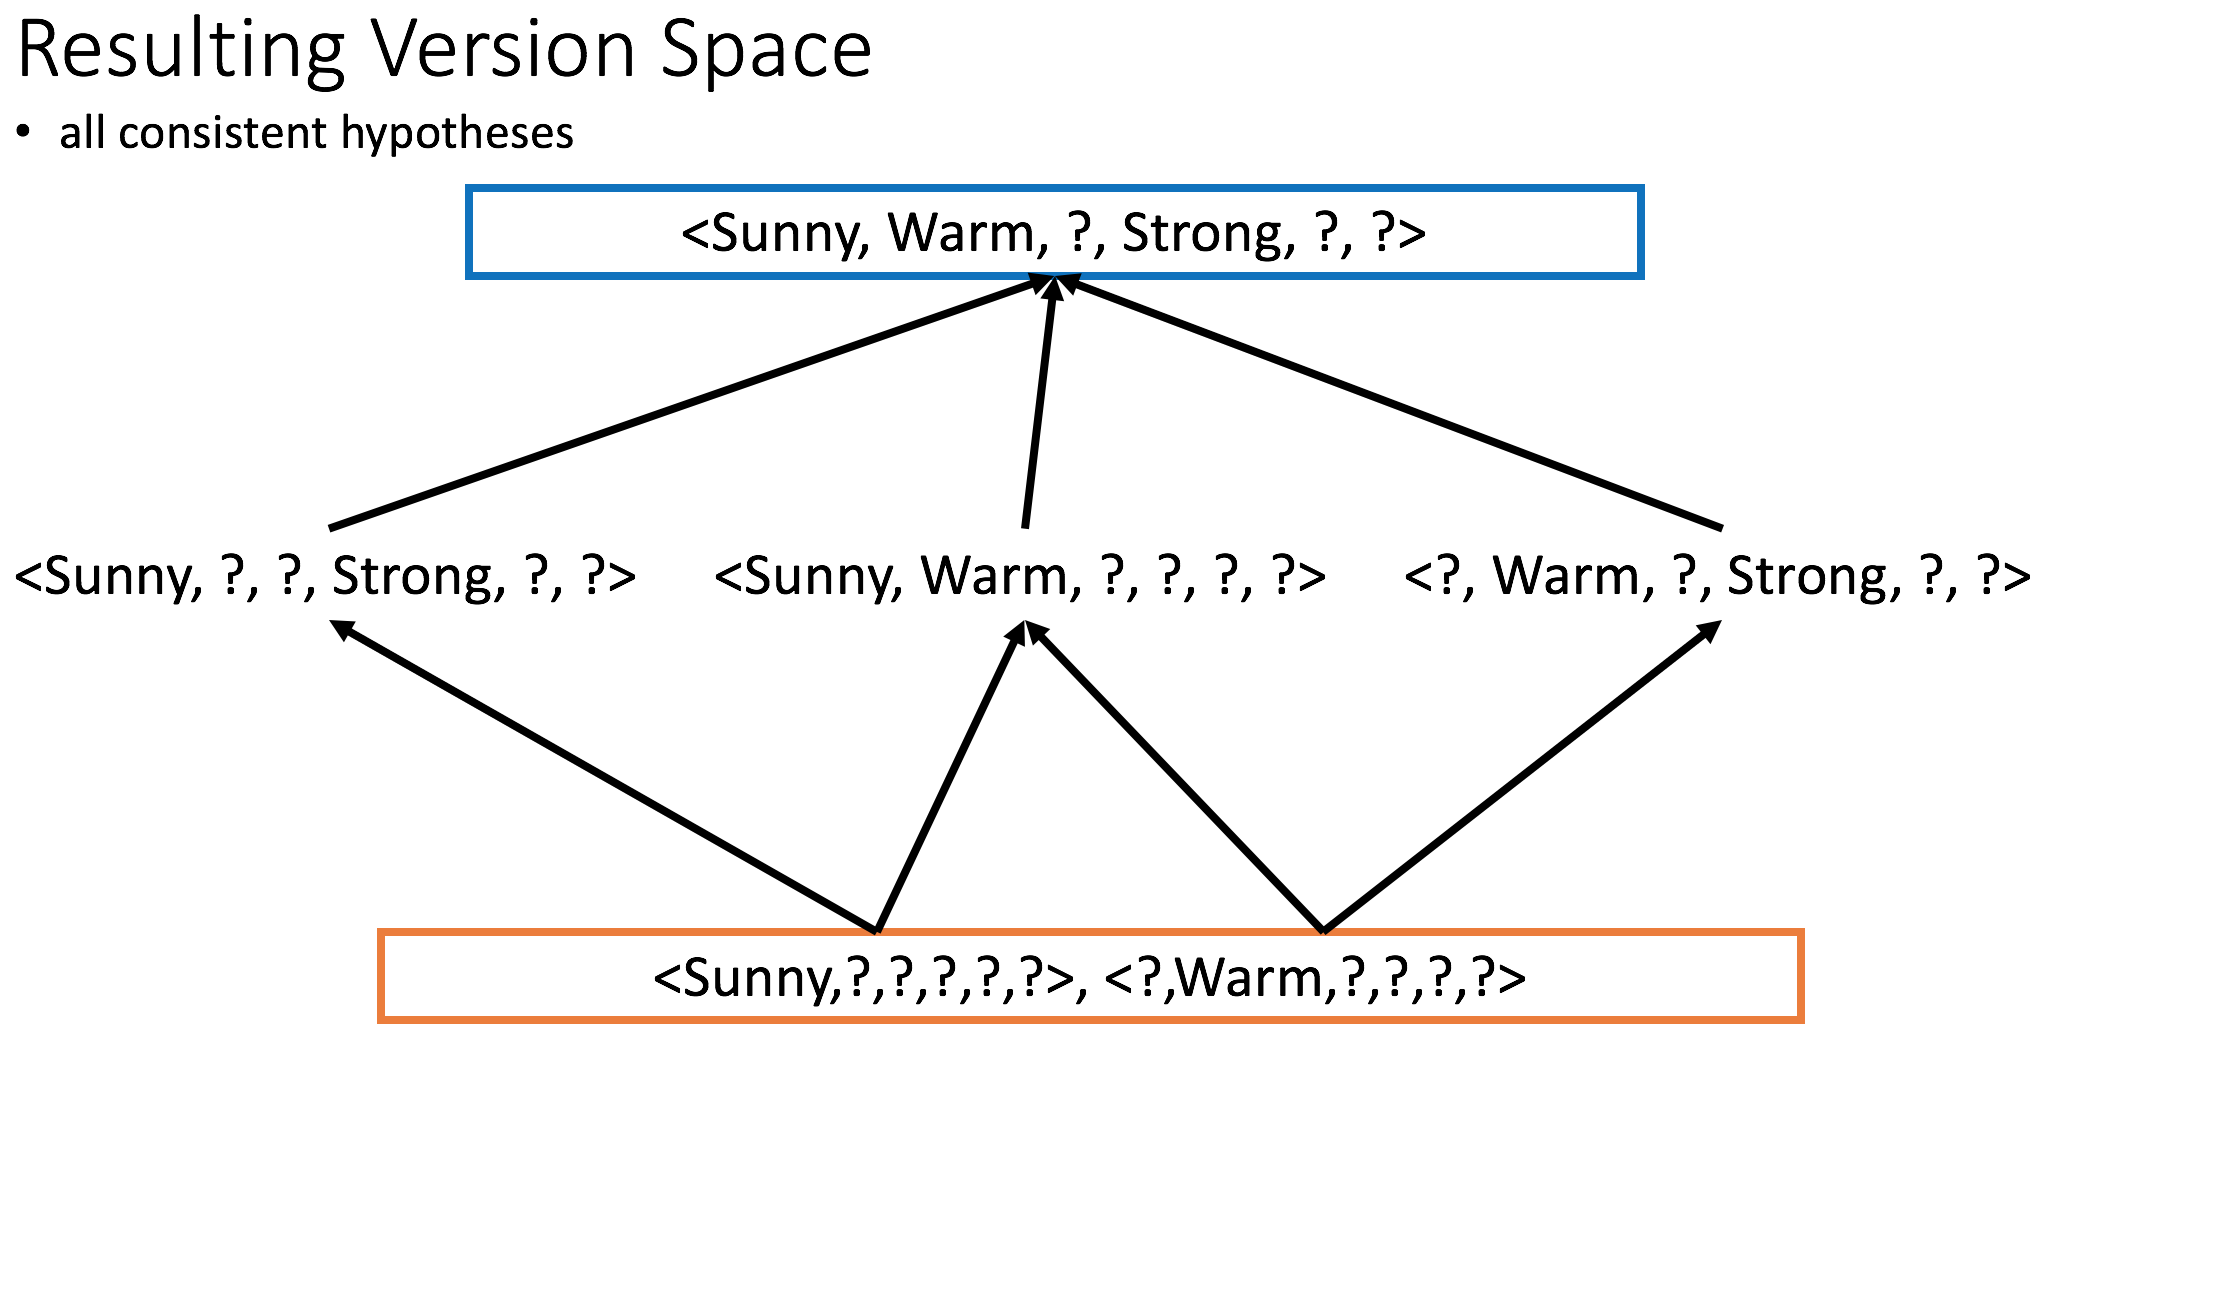
\includegraphics[width=1.1\textwidth]{cea_7}
\end{frame}

\begin{frame}{Candidate Elimination Algorithm Summary}
\textbf{Summary:}

\begin{itemize}
\item the version space learned by the algorithm converges toward the hypothesis correctly describing the target concept given:
	\begin{itemize}
	\item there are no errors in the training samples
    \item there is some hypothesis in H that correctly describes the target concept
	\end{itemize}
\end{itemize}

\end{frame}

\begin{frame}{Candidate Elimination Algorithm Summary(2)}
\textbf{Advantages}:
\begin{itemize}
\item instances don't have to be stored (lazy-learning)
\item convergence is determinable (S=G) 
\item data-efficient
\end{itemize}

\textbf{Disadvantages:}
\begin{itemize}
\item consistent samples required
\item noisy  data problematic
\item target concept must be represented by hypothesis space
\end{itemize}

In semi-supervised learning: optimal query strategy is to request instances that satisfy half the hypotheses in the current VS
\end{frame}

\subsection{Inductive Learning and Biases}


\begin{frame}{Inductive Learning}
What has been shown is associated with \emph{inductive learning}
\begin{block}{Induction}
Plausible conclusion to the general given an input (specific).
\end{block}
\begin{block}{Deduction}
Logical reasoning from given knowledge (e.g. rules).
\end{block}
\end{frame}


\begin{frame}{Inductive Learning Hypothesis}
Inductive learning makes one \textbf{fundamental assumption:}
\begin{block}{Induction Learning Hypothesis}
Any hypothesis found to approximate a target function well over a sufficiently large set of training examples will also approximate a target function well over unknown samples.
\end{block}
\textbf{$\Rightarrow$ The success of learning an inductive learning machine is heavily dependent on the provided data}
\\\textbf{$\Rightarrow$ it can at best guarantee that the output hypothesis fits the target concept over the training data.}
\end{frame}

\begin{frame}{Inductive Learning Hypothesis}
\begin{itemize}
\item problem: \\target concept might not be contained in the hypothesis space
\item solution(?):\\use hypothesis space that includes all possible hypotheses
\end{itemize}
\end{frame}


\begin{frame}{Inductive Learning Hypothesis}
\begin{itemize}
\item problem: \\target concept might not be contained in the hypothesis space
\item solution(?):\\use hypothesis space that includes all possible hypotheses
\end{itemize}
\begin{block}{Fundamental Property of Inductive Inference:}
An inductive learning machine that makes no a-priori assumptions about the identity of the target concept has no rational basis for classifying unseen instances.
\end{block}
See \cite{mitchell1997a} for an example of the futility of bias-free learning.
\end{frame}

\begin{frame}{Inductive Learning Hypothesis(2)}
\begin{block}{Inductive bias of the Candidate Elimination algorithm}
The target concept is contained in the hypothesis space and the concept could be represented by a conjunction of attribute values.
\end{block}
\end{frame}

\begin{frame}{Biases}

\begin{block}{General Bias}
Specification after which hypotheses are constructed. For example: classification accuracy, costs for storing hypotheses, human readability etc.
\end{block}

\begin{block}{Hypothesis Space Bias}
What could this be?
\end{block}

\begin{block}{Preference Bias}
What could this be?
\end{block}
\end{frame}


\begin{frame}{Biases}

\begin{block}{General Bias}
Specification after which hypotheses are constructed. For example: classification accuracy, costs for storing hypotheses or human readability
\end{block}

\begin{block}{Hypothesis Space Bias}
An hypothesis belongs to a restricted space of hypotheses, e.g. boolean conjunctions, linear threshold functions or 3-nearest neighbor
\end{block}

\begin{block}{Preference Bias}
There exists an order within the hypothesis space, e.g. prefer hypotheses with fewer disjunctions or prefer smaller decision trees
\end{block}
\end{frame}


\begin{frame}{Biases (2)}
Adjusting for the \textbf{Hypothesis Space Bias:}
\begin{itemize}
\item good classification might require complex hypothesis
\item might result in overfitting
\end{itemize}

Adjusting for the \textbf{Preference Bias:}
\begin{itemize}
\item choose an hypothesis that correctly classifies as many samples as possible
\item misclassification might be taken into account
\end{itemize}
\end{frame}


\section{Learning Theory}
\subsection{VC-Dimension}

\begin{frame}{Two central questions}
\begin{itemize}
\item Recap: inductive learning hypothesis states that any hypothesis that approx. a target function well over train data will also approx it well over unknown examples
\item Now: is there a way 
  \begin{itemize}
  \item \textbf{to quantify a (classification) model's test error over unseen data?}
  \item \textbf{that yields the amount of data necessary to learn?}
  \end{itemize}
\item Vapnik-Chervonenkis (VC) theory can help us here \cite{VapnikV.N.Chervonenkis1971}
\item PAC (probably approximately correct) not addressed here
\end{itemize}
\end{frame}

\begin{frame}{Definition}
A measure of the \textbf{capacity} of the hypothesis space that can be learned by a classification model.
\begin{block}{VC-Dimension}
The cardinality of the largest set of points that a classification algorithm can \emph{shatter}.
\end{block}

\begin{itemize}
\item Assume a binary data separation problem. What does \emph{shatter} mean? 
\item Intuitively described:
\item $\implies$  all +/- label combinations of a fixed set of points can be separated with the classifier
\end{itemize}
\end{frame}





\begin{frame}{Example: VC dimension 3}
\centering
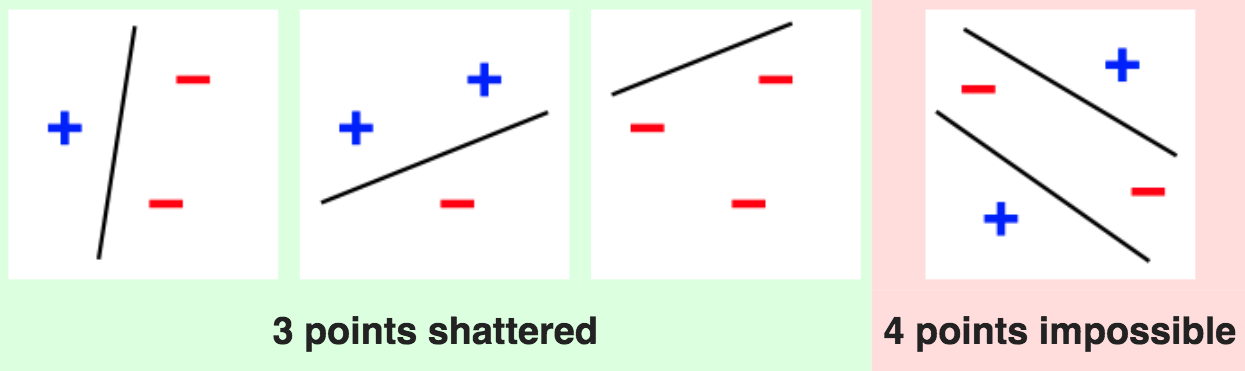
\includegraphics[width=0.9\textwidth]{shatter}\\
from \cite{WikiVCDim}

\begin{itemize}
\uncover<2->{\item to show the VC dimension is $\geq$ a number:
  \begin{itemize}
  \item $\exists$data points $\forall$labelings $\exists$hypothesis
  \end{itemize}}
\uncover<3->{\item to show the VC dimension is \textbf{not} $\geq$ a number: 
  \begin{itemize}
  \item $\forall$data points $\exists$labelings $\neg(\exists$hypothesis)
  \end{itemize}}
\uncover<4->{\item showing the lower bound is easier than showing higher bound}
\uncover<5->{\item Question: which arrangement of 3 points cannot be shattered in a binary classification problem?}\\
\uncover<6->{$\implies$3 collinear points}
%%hint: if there's time, use example from video as exercise on the board: https://www.youtube.com/watch?v=SDrFK7NxKF8

\end{itemize}
\end{frame}


\begin{frame}{Implications}
\centering
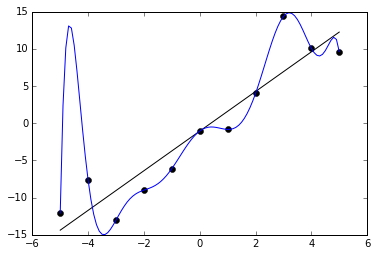
\includegraphics[width=0.5\textwidth]{overfitting}\\
from \cite{WikiOverfitting}
\begin{itemize}
\item \textcolor{blue}{VC(H)} high capacity
\item VC(H) low capacity
\item assumption: the higher VC(H) the better the classification model
\uncover<4->{\item $\implies$ wrong}
\end{itemize}
\end{frame}


\begin{frame}{Implications}
the VC dimension can predict a probabilistic \textbf{upper bound} on the test error:
\begin{equation*}
Pr\bigg(test error \leq training error + \sqrt[]{...\frac{VC(H)}{N}...}\bigg) = 1-\delta
\end{equation*} 
while $N$ being the size of the training set, $VC(H)$ the VC dimension of the family of hypotheses $H$ and $0\leq\delta\leq1$.
What are the implications?
\end{frame}



\begin{frame}{Implications}
\begin{equation*}
Pr\bigg(test error \leq training error + \sqrt[]{...\frac{VC(H)}{N}...}\bigg) = 1-\delta
\end{equation*} 

\uncover<1->{Without going much into the details, it follows:
\begin{itemize}
\item as more data is added the lower the error of the model will become}
\uncover<2->{\item the more complex the model is the more data is required to generalize well}
\uncover<3->{\item amount of data is linear to the VC dimension $\implies$ this is one reason why deep neural nets require so much data}

%hint: in practice, deep learning works better than VC dimension analysis claims, which is a shortcoming of VC dimension analysis. Also might give us the idea that we don't know why deep learning works after all. VC analysis seems unable to provide an answer here.
\end{itemize}
\uncover<4->{\textbf{main takeaway}: if you use a complex algorithm you will require a lot of data to generalize well}
\end{frame}




\newpage
\bibliographystyle{apalike}
\bibliography{lecture/bibliography.bib}

\end{document}
